\chapter{Desarrollo}
\label{chap:desarrollo}

\drop{C}{  omo} ya se ha comentado antes, el desarrollo de este proyecto ha supuesto un reto importante ya que las tecnologías utilizadas eran totalmente desconocidas. En este capítulo se explica el proceso seguido a lo largo de su desarrollo, además de presentar los principales problemas encontrados y las soluciones con las que se han abordado.

Para cada entrega se incluirán los bocetos realizados para los modelos, además del modelo renderizado en Unity, y uno de los fragmentos de código desarrollado que se considere más interesante, además de los diagramas pertinentes que ayuden a entenderlo.

Además, como algunos de los elementos desarrollados en una entrega sufrieron cambios en las siguientes, solo se explicará la versión final, por lo que puede que algo de lo explicado para una entrega no corresponda exactamente con lo enseñado en el vídeo de la misma.

Aunque algunas de las tareas de modelados de las salas han sido bastante complejas, como este trabajo no pretende centrarse en ellas la mayoría se obviarán y en su lugar se hablará de tareas más técnicas relacionadas con el diseño y la programación del código.

Por otro lado, como la naturaleza de este proyecto hace que sea muy visual, pero tampoco se pretende llenar este capítulo de capturas de pantalla de cada elemento, se deja al lector el consultar estos vídeos para ver cada uno de los elementos en acción.

\section{Entrega 0}

El objetivo de esta primera entrega fue, por un lado, establecer la estructura principal del proyecto y esbozar una primera versión del a narrativa y por otro realizar una primera toma de contacto con el desarrollo de Unity, las tecnologías \acs{VR} e instalar y configurar el entorno de desarrollo para poder empezar a trabajar en la siguiente entrega.

\subsection{Estructuración del proyecto}

El primer paso lógico tras proponer al tutor de este \acs{TFM} el proyecto y ser aprobado fue empezar a definirlo. Para ello, y partiendo de la idea principal de desarrollar una experiencia de juego haciendo uso de tecnologías \acs{VR} que pusiera en contacto con el mundo del arte a personas que suelen y no visitar museos, se generó el documento que puede verse en el anexo \ref{anexo:guia-salas}. 

Este documento comienza a detallar la narrativa del juego y la integra en una visita por un museo ficticio y, aunque terminó por sufrir varios cambios importantes, sirvió para definir el punto de partida del proyecto.

A lo largo de este documento se intenta crear una historia interesante para el jugador al mismo tiempo que generar un museo ficticio pero realista y coherente en el que se pueda desarrollar dicha narrativa. Para ello, se ha seguido el orden cronológico por las épocas más importantes en la historial de arte, definiendo una sala con una historia diferente para cada una.

A la hora de elegir los cuadros que se mostrarían en las salas se intentó buscar aquellos más representativos de su época. Para ello, se contó con el asesoramiento de una historiadora del arte, que ha sido quien ha dado el visto bueno al rigor artístico del museo y sus salas.

\subsection{Primera toma de contacto con Unity}

A continuación se presenta un resumen de la interfaz de Unity para que el lector pueda entender algunos de los conceptos de los que se hablará más adelante.

\begin{figure}[!h]
\begin{center}
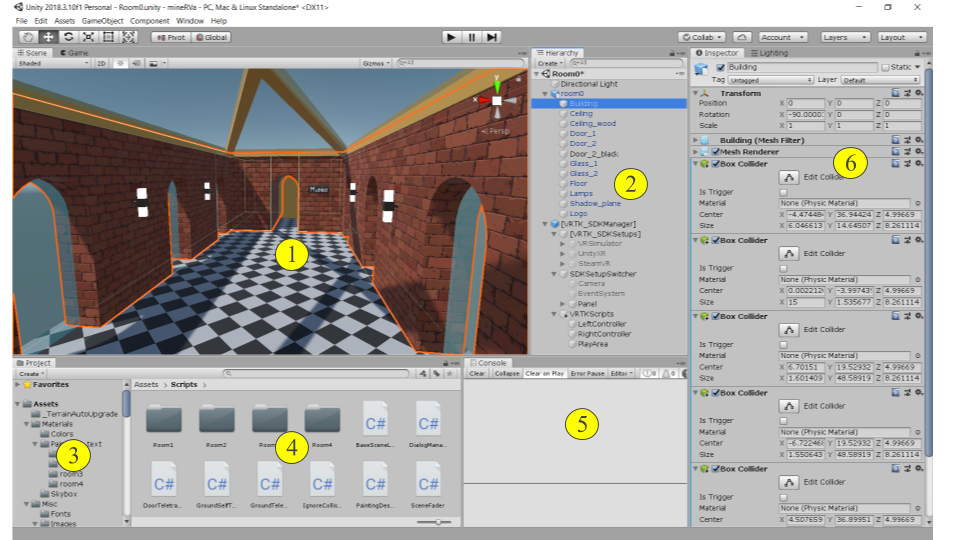
\includegraphics[width=1\textwidth]{imagenes/7/interfaz-unity.png}
\caption{Resumen de la interfaz de Unity}
\label{fig:interfaz-unity}
\end{center}
\end{figure}

\begin{enumerate}
    \item Vista de la escena actual, en la que el usuario puede obtener una vista previa de la escena e interactuar con los objetos tridimensionales para colocarlos. Funciona de manera parecida a Blender.
    
    \item Vista de la jerarquía de la escena, en la que pueden verse los objetos que hay y sus relaciones; por ejemplo, si están emparentados.
    
    \item Vista del inspector en la que aparece la información de los componentes de un objeto seleccionado. Un componente puede ser prácticamente cualquier cosa desde un script a un material.
    
    \item Vista del proyecto, donde aparecen todas las carpetas disponibles.
    
    \item Vista donde aparecen los elementos de la carpeta seleccionada. En este caso, pueden verse algunos de los scripts con los que se ha trabajado.
    
    \item Consola de salida en la que aparece información del proyecto.
\end{enumerate}

\subsection{Configuración del entorno de desarrollo}

Antes de poder empezar a desarrollar el proyecto fue necesario elegir un \acs{IDE} y un framework con el que trabajar. Como ya se ha explicado en los capítulos \ref{chap:estado_arte} y \ref{chap:tecnologia}, tras comparar las ventajas y desventajas de los entornos de desarrollo y librerías disponibles en el mercado se decidió trabajar con Unity, el framework \acs{VRTK} y la librería SteamVR para lo que, tras instalarlas, hubo que importarlas manualmente al proyecto de Unity.

La principal motivación de usar este framework es toda la configuración por defecto que trae; de no haber utilizado estas librerías, hubiera sido necesario implementar de 0 un sistema de Realidad Virtual interactivo, lo que hubiera sido un \acs{TFM} por si mismo. En cambio, ha sido posible importar directamente y con relativa poca configuración un sistema funcional preparado para trabajar con él.

Por otro lado, en lo que respecta al movimiento y desplazamiento del usuario, se presentaron dos vertientes.

\begin{itemize}
    \item Utilizar el \textbf{joystick} de los mandos para moverse, como si de un juego clásico se tratara. El problema de este enfoque es que genera \textbf{mareos} en los jugadores, ya que cuando los ojos detectan un movimiento que el sistema de equilibro no se genera una sensación muy incómoda que obliga al jugador a parar inmediatamente de jugar. En mi caso, por ejemplo, intenté jugar al \textit{Pavlov VR}, un juego que implementa este modelo, y apenas pude jugar tres minutos antes de tener que parar y tumbarme.
    
    \item En contraposición, el modelo que están implementando la mayoría de juegos \acs{VR} es de \textbf{lanzar} a los jugadores, quienes utilizan el joystick para apuntar al sitio donde quieren moverse, como si de una catapulta se tratase, y se teletransportan al lugar indicado, evitando por completo los mareos. 
\end{itemize}

Por tanto, se ha elegido el segundo modelo para utlizar en este juego.

\section{Entrega 1}

Como se indicó en el capítulo \ref{chap:plan_entregas}, el objetivo final de las iteraciones de esta entrega fue aprender a importar modelos a Unity desde Blender y diseñar e implementar el tutorial del proyecto y que éste fuera completamente funcional. 

\subsection{Modelado e importación}

Lo primero que se hizo antes de comenzar a modelar en Blender, ya que es mucho menos productivo empezar a trabajar sin una idea previa, fue diseñar un boceto en papel en el poder basar el modelado posterior.

Como se consideró que el museo sería más realista si en lugar de empezar directamente en él el jugador tuviera que recorrer un pequeño pasillo que funcionara de antesala y desde el que se pudiera ver el exterior, fue el primer boceto que se hizo, y tras él se dibujó la sala que actuaría de tutorial. Además, en esta antesala se recibiría una llamada de la directora del museo en la que presenta al jugador como un detective de renombre y expone el problema del cuadro robado. Tras ello, le indicaría que hablase con el vigilante del museo para más información.

Tras ello, en la primera sala se tendría que presentar un cuadro muy reconocible y una pequeña prueba relacionada con él, por lo que se decidió utilizar el cuadro \textit{El Hijo del Hombre} de René Magritte (1964) y que el jugador tuviera que cambiar de sitio una pieza de fruta relacionada con este cuadro, de este modo aprendiendo que puede interaccionar con los elementos virtuales y que habrá relación entre las pruebas y las obras de arte de tal manera que el reto sea darse cuenta de estas ideas y no la propia prueba en sí, ya que sería algo trivial. La imagen \ref{fig:bocetos-salas-0-1} muestra el boceto de estas dos salas, que fue dibujado antes de comenzar a modelarlas.

\begin{figure}[!h]
\begin{center}
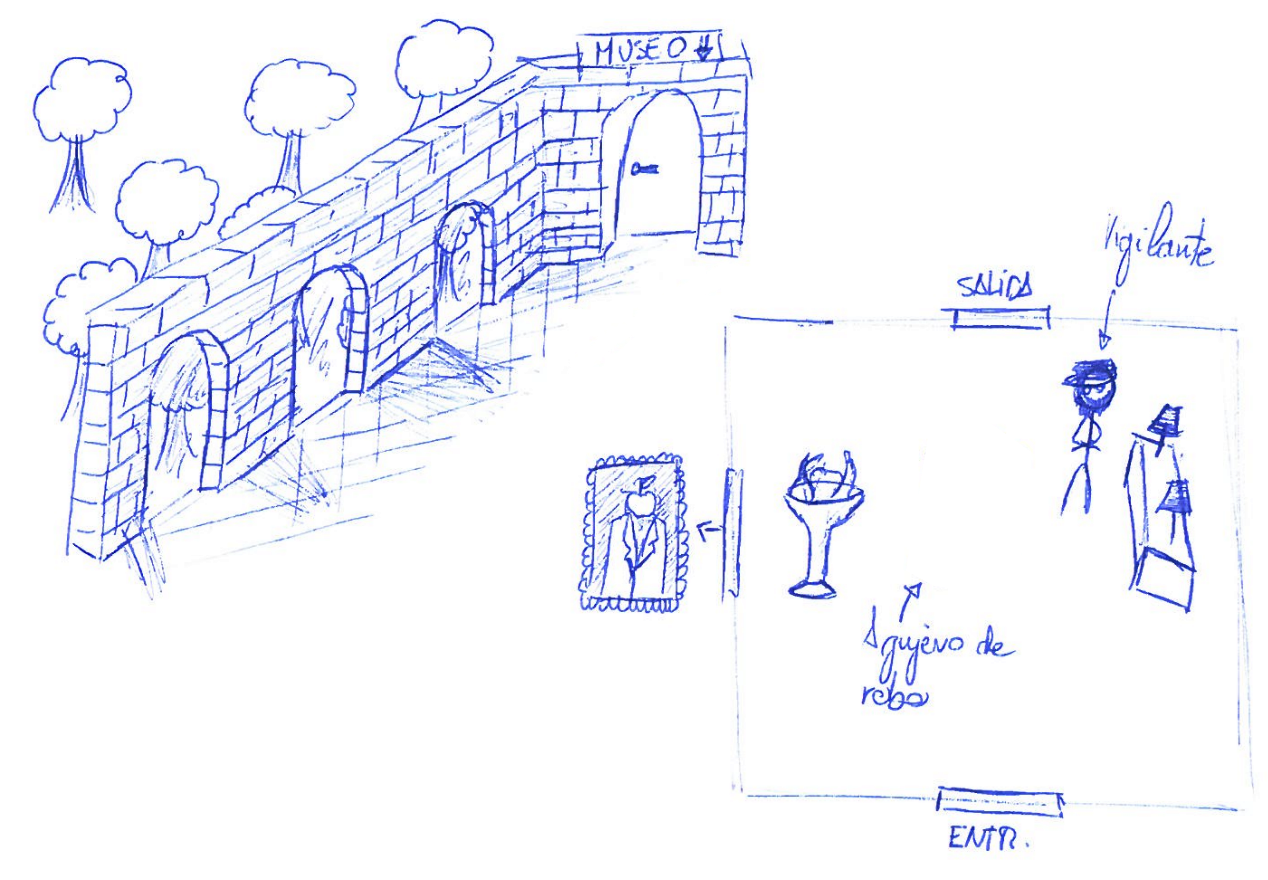
\includegraphics[width=.8\textwidth]{imagenes/7/bocetos/boceto-sala-0-1.png}
\caption{Boceto de la antesala y la sala de tutorial}
\label{fig:bocetos-salas-0-1}
\end{center}
\end{figure}

Una vez terminados los bocetos, se modeló la primera sala en Blender se comenzó a trabajar en importarla desde Unity, para lo que es necesario crear una Escena e importar en ella el archivo Blender desde el gestor de archivos. Una vez que lo hagamos, aparecerá como un \textbf{Prefab}\footnote{\url{https://docs.unity3d.com/es/current/Manual/Prefabs.html}}. De este modo, cuando el archivo Blender se modifique Unity lo detectará y actualizará su copia local, aunque por ser un Prefab no pueden modificarse desde Unity sin perder esta propiedad.

Actualmente, Blender cuenta con dos motores de renderizado; Blender Internal y Blender Cycles, y no son compatibles entre sí. Esto quiere decir que si por ejemplo creamos un material en Blender Internal y luego cambiamos a Cycles, éste no aparecerá. Aunque en teoría Unity trabaja mejor con los materiales de Blender Internal, al importarlos no aparecen como deberían y no pueden modificarse sus propiedades como su color, su \textit{metalicidad} o su mapa de normales, por lo que ha sido necesario rehacer todos los materiales de los modelos y volver a aplicarlos a mano.

Vamos a tomar como ejemplo una de las paredes de ladrillos para ver el flujo de trabajo de los materiales; tras modelarla, habría que descargar una textura para ella, para lo que se ha utilizado el sitio web \url{https://3dtextures.me/} que proporciona texturas procedurales gratuitas y con mapas de normales y rugosidad con licencia libre. Una vez hecho, se crea un material en Blender al que se le aplica la textura para ver cómo quedaría, aunque Blender Internal no da la opción de añadir más mapas a la textura. Tras esto, se importa el modelo desde Unity y se crea un nuevo material, con la misma textura, al que se le añaden y configuran el resto de mapas.

La imagen \ref{fig:unity-sala-0} muestra el resultado final del modelado y la importación a Unity. Como el exterior con árboles, que puede verse a través de las ventanas, se reutiliza en otras salas se ha movido a una escena aparte que se importa cuando es necesario, recudiendo de este modo el peso de los modelos.

\begin{figure}[!h]
\begin{center}
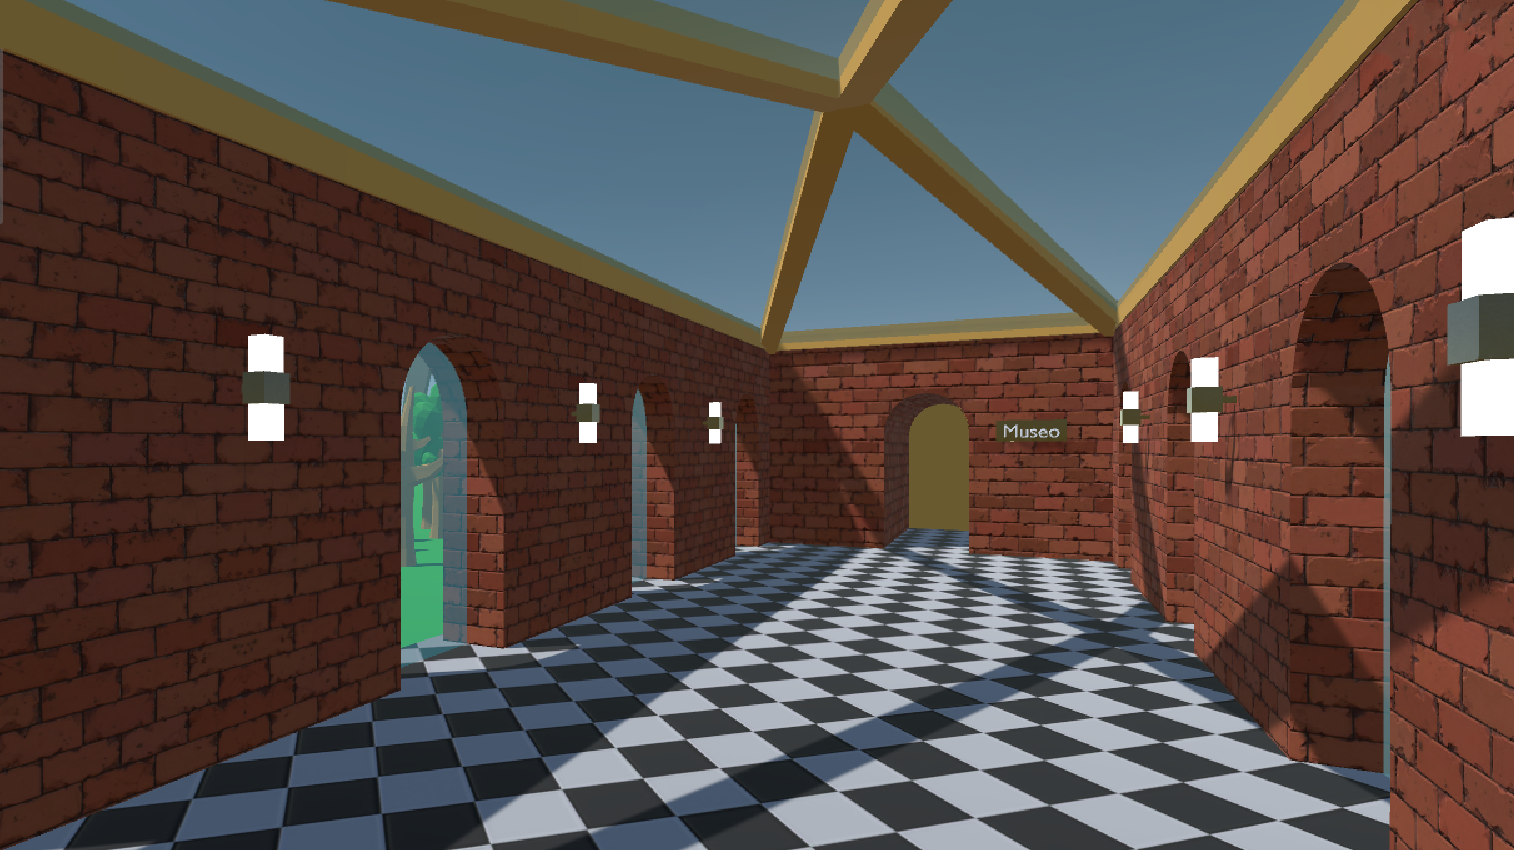
\includegraphics[width=0.85\textwidth]{imagenes/7/salas-unity/unity-sala-0.png}
\caption{Sala 0 renderizada en Unity}
\label{fig:unity-sala-0}
\end{center}
\end{figure}

Tras ello se hizo lo mismo con la sala de tutorial, que puede verse en la figura \ref{fig:unity-sala-1}. Para dar a entender al jugador que están relacionadas, se ha utilizado la misma textura de ladrillos para las paredes y el mismo techo de cristal, lo que ayuda a aumentar la claridad y dar una sensación de amplitud,

\begin{figure}[!h]
\begin{center}
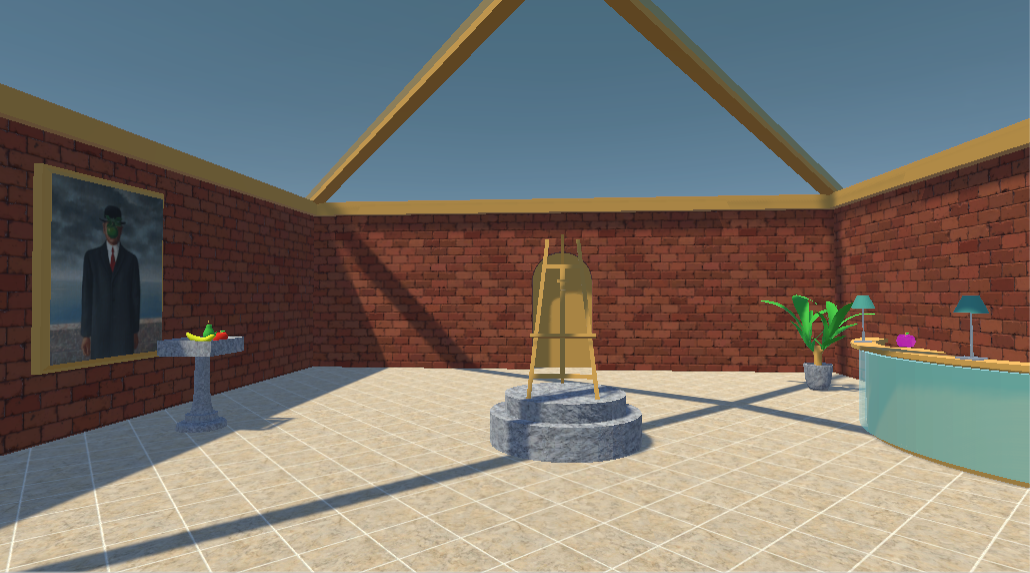
\includegraphics[width=0.85\textwidth]{imagenes/7/salas-unity/unity-sala-1.png}
\caption{Sala 1 renderizada en Unity}
\label{fig:unity-sala-1}
\end{center}
\end{figure}

Además, aunque las cajas de colisiones automáticas de Unity funcionan bien para objetos no lo hacen para habitaciones, ya que estas cajas la rodean y no permiten detectar colisiones interiores. Por ello, ha sido necesario definir manualmente estas colisiones, para lo que se han utilizado los componentes \texttt{Box Collider} para cada una de la paredes, el techo y el suelo. Estas cajas de colisiones definen los \textit{limites físicos} de los objetos e impiden que el jugador los atraviese.

\subsection{Viajar entre salas}

Una escena en Unity es una unidad que permite incluir en ella elementos que estén estrechamente relacionados desde el punto de vista del juego, como modelos o scripts. Desde la documentación de Unity se anima al desarrollador a encapsular cada nivel del juego en una escena; así, la equivalencia que se ha usado en este proyecto es de una sala por escena.

Una vez que las dos salas estaban modeladas se trabajó en hacer que el jugador pudiera viajar entre ellas; para ello, se escribió un script en C\# que permite cambiar la escena actual a otra cuando el jugador toque una puerta 

Para ello, lo primero que se hizo fue añadir una caja de colisiones sin físicas a la puerta, lo que permite añadir un \textit{listener} para detectar colisiones y poder activar otras funciones. Tras ello, se desarrolló y añadió un script como componente, que puede verse simplificado en el listado \ref{lst:viajar-salas}, que usa la clase \texttt{SceneManager} para cambiar la escena cuando el jugador colisiona con ella tras comprobar previamente que no se encuentra cargada. En él se declaran dos variables públicas para poder definirlas desde el propio inspector de Unity más cómodamente, como puede verse en la figura \ref{fig:door-teleporter-inspector}, lo que añade flexibilidad y reutilización al código. El script entero se encuentra en el archivo \texttt{DoorTeletransporter.cs}.

\begin{lstlisting}[caption=Fragmento del script para viajar entre salas, label=lst:viajar-salas]
public string sceneName;
public float fadingTime = 10.0f;

private void OnTriggerEnter(Collider other)
{
    if (sceneName != String.Empty && !SceneManager.GetSceneByName(sceneName).isLoaded)
    {
        SceneManager.LoadScene(sceneName, LoadSceneMode.Single);
    }
}
\end{lstlisting}

\begin{figure}[!h]
\begin{center}
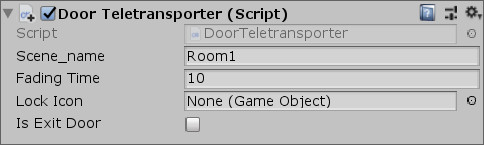
\includegraphics[width=0.6\textwidth]{imagenes/7/door-teleporter-inspector.jpg}
\caption{Script para cambiar de salas desde el inspector}
\label{fig:door-teleporter-inspector}
\end{center}
\end{figure}

Además, Unity utiliza la convención \textit{CamelCase} para nombrar sus variables, que es un estilo de escritura que se aplica a frases que omite los espacios y hace que cada palabra empiece en mayúsculas . Por ello, si la implementamos en nuestro código es capaz de reconocerlo y representar el nombre de las variables en el inspector correctamente.

Por otro lado, cada script puede implementar dos funciones, \texttt{Start()} y \texttt{Update()}, que se ejecutan automáticamente al inicio de la escena y en cada frame, respectivamente. Este paradigma es totalmente distinto a la programación lineal, ya que es necesario realizar cualquier cambio de manera iterativa; por ejemplo, si queremos mover un objeto un metro durante un segundo, deberemos parametrizar las distancias y los tiempos para que esta posición se actualice, aproximadamente, sesenta veces cada segundo.

\subsection{Interacción con objetos virtuales}

Una vez modeladas las dos salas, se comenzó a trabajar en hacer que el jugador pudiera interactuar con los objetos virtuales. Al estar utilizando el framework \acs{VRTK} se han podido hacer uso de sus funciones para facilitar mucho el trabajo.

Lo primero que se hizo, tras modelar las tres piezas de fruta (una manzana, un plátano y una pera) e importarlas a Unity fue dotarlas de físicas, para lo que se utilizaron los componentes \texttt{Box Collider} para definir sus límites y \texttt{Rigidbody} para hacerlas responder a la gravedad. Tras ello se hizo que interactuaran con los mandos del jugador con ayuda de los componentes \texttt{VRTK\_Interactable\_Object}, \texttt{VRTK\_Child\_Of\_Controller}, \texttt{VRTK\_Interact\_Haptics} y se hizo que apareciera un borde amarillo cuando su caja de colisión detectara el mando con ayuda del componente \texttt{VRTK\_-} \texttt{Outline\_Object\_Highlighter}. Tras ello, se utilizó una \textit{snap drop zone} o zona en la que poder colocar objetos, para lo que se adaptó uno de los modelos proporcionados por el framework. Tras configurarlo adecuadamente, fue posible colocar sobre esta zona piezas de fruta y que estas automáticamente adquirieran la posición y rotación adecuadas.

Lo que se explica a continuación no se hizo hasta dos entregas posteriores, pero se contará ahora por estar estrechamente relacionado con ello. Para evitar que el jugador saliese de la sala sin hacer caso al vigilante, se añadió un script a la \textit{snap drop zone} antes mencionada que detectara cuando el jugador dejaba un objeto con la etiqueta \texttt{Apple} para desbloquear la puerta. Por un lado, para conseguir detectar cuando el jugador colocaba objetos en la zona se añadió un \textit{listener} al evento \texttt{ObjectSnappedToDropZone}, emitido por el componente \texttt{VRTK\_SnapDropZone}, que permite saber programáticamente cuándo ocurre esto. Por otro, para desabilitar la puerta y evitar que el jugador viaje entre salas, se desabilita por defecto su caja de colisiones y solo se vuelve a activar cuando el jugador coloca la manzana en su sitio. Más adelante también se utilizaría este sistema para activar uno de los diálogos del vigilante que felicitase al jugador por haberlo hecho bien.

Como resultado de esta entrega se generó el primer entregable y, por tanto, se grabó un vídeo presentando el proyecto y enseñando los avances, que puede verse en el siguiente enlace.

\begin{center}
    \url{https://youtu.be/m7rvcdZuUMI}
\end{center}



\section{Entrega 2}

La segunda entrega del proyecto estuvo más centrada en el modelado que la primera, concretamente en la sala del gótico. Tras diseñar el boceto de la misma, que puede verse en la figura \ref{fig:bocetos-sala-2}, se modeló el Blender. Al ser un modelo lleno de detalles y diseños y formas muy específicos, como los arcos o las ventanas, se tardó bastante en terminar. El resultado final puede verse en la figura \ref{fig:unity-sala-2}.

\begin{figure}[!h]
\begin{center}
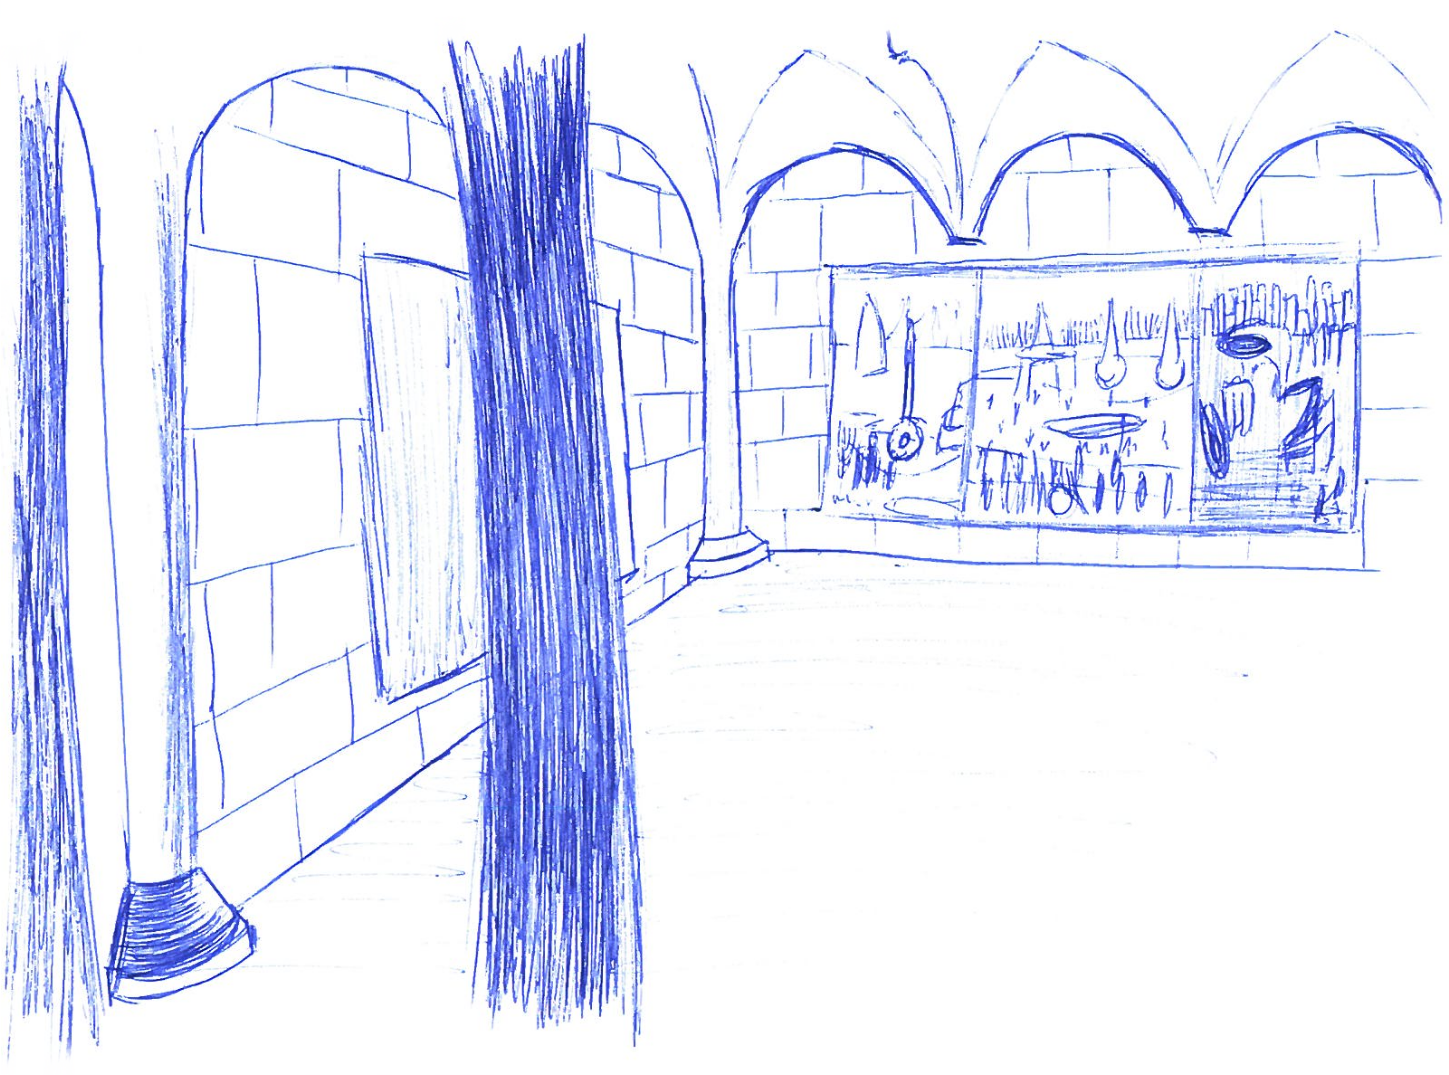
\includegraphics[width=0.75\textwidth]{imagenes/7/bocetos/boceto-sala-2.png}
\caption{Boceto de la segunda sala}
\label{fig:bocetos-sala-2}
\end{center}
\end{figure}

\begin{figure}[!h]
\begin{center}
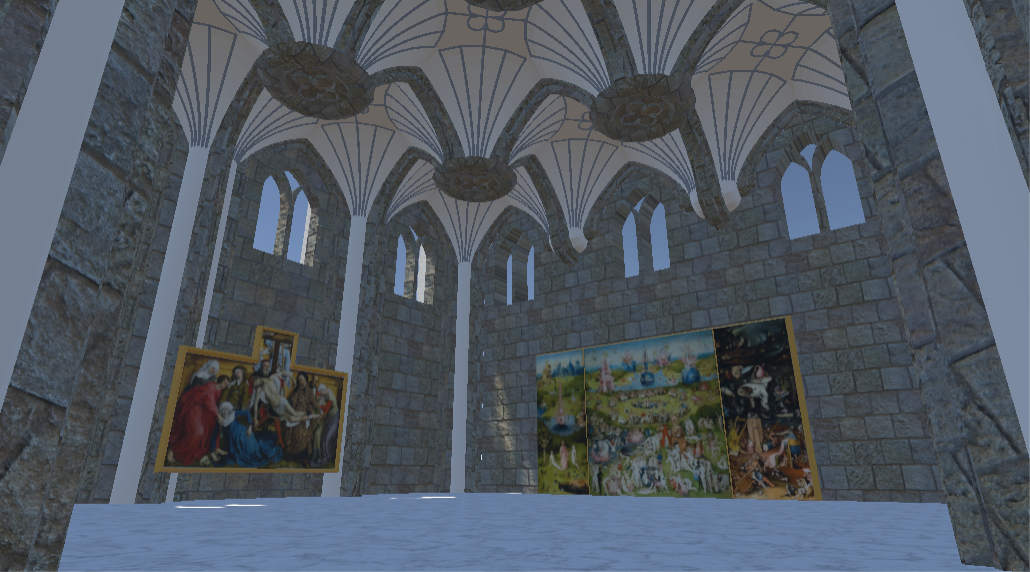
\includegraphics[width=0.85\textwidth]{imagenes/7/salas-unity/unity-sala-2.png}
\caption{Sala 2 renderizada en Unity}
\label{fig:unity-sala-2}
\end{center}
\end{figure}

\subsection{Activación de una palanca virtual}

Una vez se contaba con el modelo, se pasó a implementar la prueba. Para esta sala se decidió esconder una palanca tras uno de los cuadros laterales que, al activarla, abriera en dos el \textit{Jardín de las Delicias}. Para ello, una vez modelado el hueco en la pared con la palanca detrás del cuadro elegido, se utilizó el script del framework \acs{VRTK} \texttt{VRTK\_ArificialRotator} y se integró con un script propio para dotar de dicha funcionalidad tanto a la palanca como a la puerta. A continuación, en la figura \ref{fig:lever-controller-inspector} puede verse un fragmento de este último script desde el inspector de Unity y cómo contiene al primero. Además, también puede verse cómo se han asignado el resto de elementos mencionados para que pueda acceder a ellos y modificarlos.

Por ejemplo, desde este script es posible definir el contenido del cuadro de texto que muestra si el cuadro está abierto o cerrado, su velocidad de apertura y la referencia a los dos lados del cuadro, que se utilizará para acceder a ellos y modificar su posición.

\begin{figure}[!h]
\begin{center}
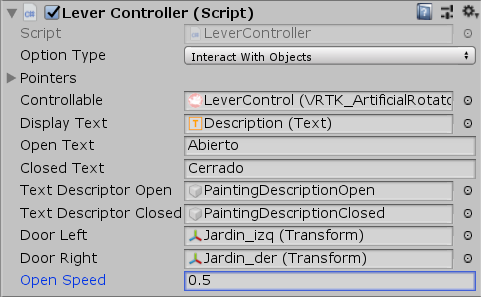
\includegraphics[width=0.6\textwidth]{imagenes/7/lever-controller.png}
\caption{Script para controlar la palanca desde el inspector}
\label{fig:lever-controller-inspector}
\end{center}
\end{figure}

A continuación, en el listado \ref{lst:lever-controller} se presenta simplificado el script utilizado para abrir y cerrar la puerta, que se puede ver completo en el archivo \texttt{LeverController.cs}. Como puede verse, todo se realiza dentro del método \texttt{Update()}, actualizando en cada frame la posición de los elementos utilizando el método \texttt{Lerp} de la clase \texttt{Vector3}, que implementa una función de interpolación lineal que permite modificar un vector tridimensional.

\begin{lstlisting}[caption=Fragmento del script para abrir y cerrar una puerta abatible con una palanca, label=lst:lever-controller]
public Transform doorLeft;
public Transform doorRight;
public float openSpeed;

private void Update()
{
    doorLeft.position = Vector3.Lerp(doorLeft.position,
                                      leftPosition,
                                      Time.deltaTime * openSpeed);
    
    doorRight.position = Vector3.Lerp(doorRight.position,
                                       rightPosition,
                                       Time.deltaTime * openSpeed);
    

}
\end{lstlisting}

Además, multiplicando la velocidad de apertura por el tiempo transcurrido desde el último frame ejecutado (obtenido con la función \texttt{Time.detaTime}) podemos asegurar que el todos los ordenadores en los que se ejecute se abrirá a la misma velocidad, evitando así que el juego se ejecute más rápido en ordenadores más potentes.

Por otro lado, para permitir al jugador abrir y cerrar el cuadro que esconde la palanca como si fuera ventana se ha utilizado el script \texttt{VRTK\_Physics\_-} \texttt{Rotator} al que, indicándole un vector que actúa como bisagra y el ángulo de apertura, además de otros parámetros, es capaz de rotar el objeto que lo contiene.

\subsection{Teletransportar los objetos que toquen el suelo}

Para evitar que el jugador tuviera que agacharse a recoger los objetos virtuales que caen al suelo (lo que puede ser peligroso, ya que con las gafas no se ve el mundo real y se puede llegar a chocar contra algún objeto), se diseñó un pequeño script que hace que cuando estos objetos chocan contra el suelo vuelvan a su posición original. Este script hace que cuando la caja de colisión de un objeto detecta un choque comprueba si es el suelo, y si sí cambia la posición de dicho objeto con la que tenía al cargar la escena, que previamente ha almacenado en una variable, automatizando la tarea.

En el listado \ref{lst:object-teletransporter} puede verse el fragmento de este script que detecta las colisiones, cambiando la posición y la rotación del objeto para que coincida con su inicial. Además, también se resetean sus velocidades iniciales y angulares, ya que si no el objeto mantiene la velocidad y la aceleración que tenía mientras caía, lo que hacía que rebotaran contra las superficies y volvieran a caer cada vez más y más rápido.

\begin{lstlisting}[caption=Fragmento del script para teletransportar un objeto si toca el suelo, label=lst:object-teletransporter]
private void OnTriggerEnter(Collider other)
{
    if (other.tag == GroundTag && instance != null)
    {
        Rigidbody rb = instance.GetComponent<Rigidbody>();

        instance.position = initialPosition;
        instance.rotation = initialRotation;
        rb.velocity = initialVelocity;
        rb.angularVelocity = initialAngularVelocity;
    }
}
\end{lstlisting}


Y por último, se comenzó a prototipar la siguiente sala, aunque como apenas se empezó en esta entrega su explicación se deja para la siguiente.

Por tanto, como resultado de esta entrega se generó una versión del proyecto que contenía la antesala y las dos primeras salas funcionalmente terminadas y un prototipo con la estructura básica de la tercera. El vídeo que enseña los avances puede verse a continuación.

\begin{center}
    \url{https://youtu.be/kfEnxP5dHU4}
\end{center}



\section{Entrega 3}

A continuación se comenzó a trabajar en la tercera entrega. Como la anterior sala se terminó y se empezó a modelar la tercera, lo primero que se hizo fue terminar el modelo de la misma. En la figura \ref{fig:bocetos-sala-3} puede verse el boceto que se dibujó antes de comenzar a modelar para tener un punto de partida.

\begin{figure}[!h]
\begin{center}
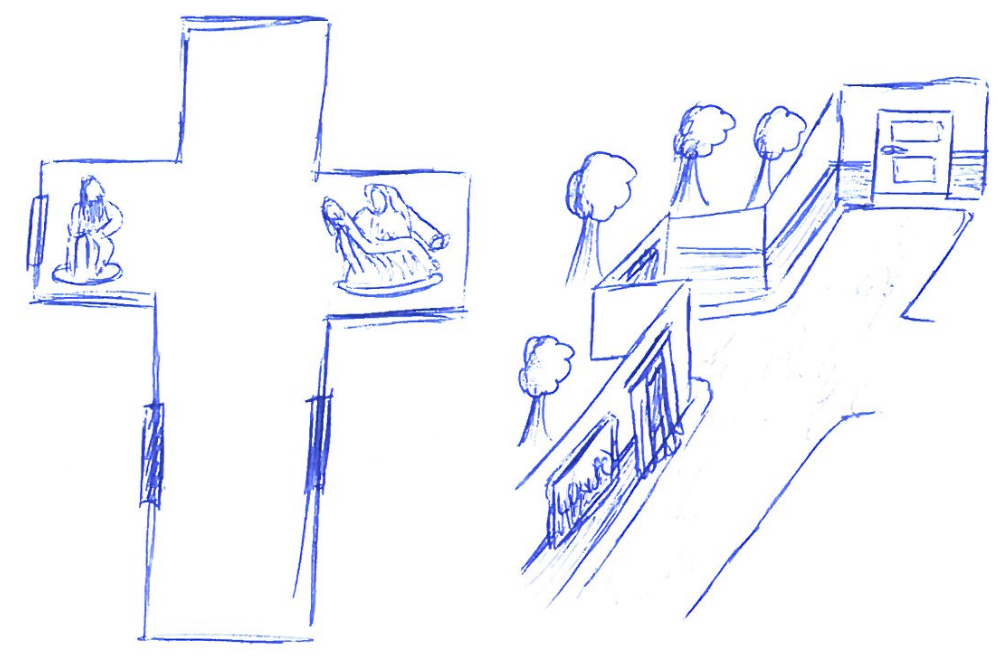
\includegraphics[width=0.75\textwidth]{imagenes/7/bocetos/boceto-sala-3.png}
\caption{Boceto de la tercera sala}
\label{fig:bocetos-sala-3}
\end{center}
\end{figure}

Más adelante, en la figura \ref{fig:unity-sala-3} puede verse la sala ya terminada e importada desde Unity. Finalmente, la prueba de esta sala consiste en ayudar al vigilante a recoger restos que otros visitantes han dejado en el museo. En concreto son 4; una lata de refresco, una botella de cristal, una taza de café y una tela que tapa uno de los cuadros. Una vez que el jugador los ha depositado todos en la papelera que puede verse al fondo, la sala se desbloquea y puede continuar visitando el museo.

\subsection{Recogiendo basura virtual}

Para hacer los elementos presentados anteriormente interactivos se utilizó un procedimiento similar a las piezas de fruta de la primera sala, utilizando la funcionalidad y las interfaces que provee el framework \acs{VRTK}. Por tanto, se omitirá su explicación y se pasará directamente a presentar el funcionamiento de la papelera.

\begin{figure}[!h]
\begin{center}
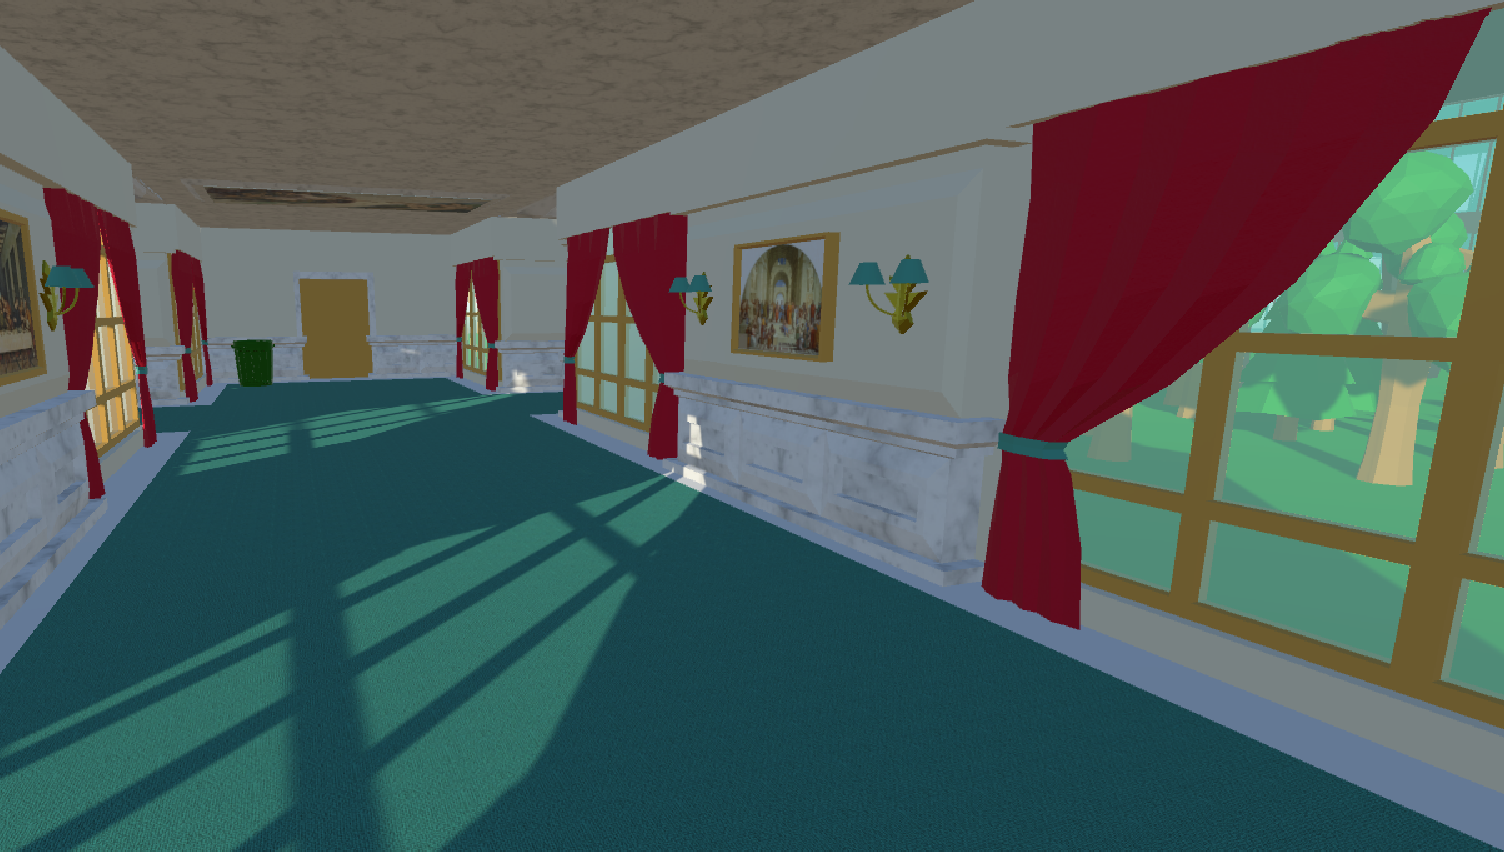
\includegraphics[width=0.85\textwidth]{imagenes/7/salas-unity/unity-sala-3.png}
\caption{Sala 3 renderizada en Unity}
\label{fig:unity-sala-3}
\end{center}
\end{figure}

Aunque inicialmente se intentaron varios enfoques para hacer funcionar esta papelera, como hacer que el jugador tuviera que depositar dentro los objetos, tras varias pruebas se vio que no siempre caían dentro, y como a estos objetos también se les añadió el script para que volvieran a su sitio al caer, el jugador tenía que volver a la posición de origen de nuevo a por ellos, lo que era bastante tedioso. Por ello, finalmente se consideró que simplemente con soltar los objetos cerca de la papelera, automáticamente se metieran dentro de ella y desaparecieran. Para ello se volvieron a utilizar las \textit{snap drop zones} de \acs{VRTK}. 

Por tanto, se colocaron cuatro zonas concéntricas, una por cada objeto, y se configuraron de tal manera que al dejar un objeto dentro hacían que su tamaño se encogiese hasta ser prácticamente invisible, y luego lo eliminaban. Por otro lado, para detectar cuándo una de estas zonas detectaba un objeto, se utilizaron eventos de Unity. Estos eventos permiten suscribirse a ellos y resultar notificado cuando se activen. Así, las \textit{snap drop zones} ofrecen sus propios eventos; por tanto, una vez podemos acceder a las 4 zonas desde el código basta con utilizar el operador \texttt{+=} para suscribir un método que implemente la interfaz necesaria al evento de un objeto.

En el listado \ref{lst:trash-detector} pueden verse simplificadas los fragmentos más relevantes de este script. La primera linea declara un vector público de \textit{snap drop zones}, lo que permite definir desde el inspector su tamaño y sus elementos. Posteriormente, cuando la escena comienza, se recorre este vector con un iterador \texttt{foreach} y se suscribe un método propio a los eventos de todas las zonas que anuncian que un objeto le ha sido agregado. Así, cada vez que una zona adquiera un objeto se llamará a la función de la línea \ref{line:check-tag}, que comprobará si el objeto añadido corresponde con aquellos que nos interesan y podrá de este modo llevar un registro de cuántos elementos se han depositado en la papelera y cuándo desbloquear la puerta de salida. 

\begin{lstlisting}[caption=Fragmento del script para detectar piezas de basura, label=lst:trash-detector, escapechar=|]
public VRTK_SnapDropZone[] snapDropZones;

private readonly string TRASH_TAG = "Trash";

private void Start()
{
    foreach (VRTK_SnapDropZone sdz in snapDropZones)
    {
        sdz.ObjectSnappedToDropZone += OnTrashSnapped;
    }
}

internal void OnTrashSnapped(object sender, SnapDropZoneEventArgs e)
{
    if (e.snappedObject.tag == TRASH_TAG)|\label{line:check-tag}|
    {
        trashCounter++;
    }
}
\end{lstlisting}

En la imagen inferior, la figura \ref{fig:trash-detector}, puede verse el script desde el inspector de Unity y cómo es posible definir de manera flexible el tamaño y los elementos del vector para que puedan ser accedidos después desde el código. 

\begin{figure}[!h]
\begin{center}
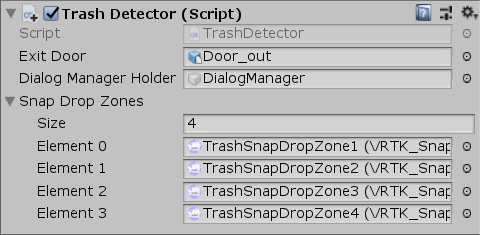
\includegraphics[width=0.6\textwidth]{imagenes/7/trash-detector.png}
\caption{Script para detectar piezas de basura desde el inspector}
\label{fig:trash-detector}
\end{center}
\vspace{-0.25cm}
\end{figure}

\subsection{Mostrando la descripción de los cuadros}

Lo siguiente en lo que se trabajó fue en mostrar la descripción de los cuadros cuando el jugador pulsara un botón. Se dedicó bastante tiempo a pensar la solución más orgánica, desde poner al lado de cada una cuadro un pequeño marco con la descripción, como en los museos de verdad, a cambiar la textura del cuadro a un texto con su descripción, pero ninguna terminaba de ser cómoda para el jugador. Por lo tanto, finalmente se decidió superponer un cuadrado semitransparente delante de la cámara con la descripción del cuadro, que apareciese y desapareciese cuando se pulsara un botón. Además, esta solución permitía reutilizarse para el sistema de diálogos que se implementaría en un futuro, y por lo tanto ahorrando tiempo de desarrollo, por lo que se decidió elegirla. Este cuadro sigue siempre al jugador pero está desactivado por defecto, por lo que solo es visible cuando se activa.

En la figura \ref{fig:camera-overlay} se muestra cómo funciona. Como puede verse, se define un cuadro delante de la cámara que copia su localización y rotación para seguirla aunque el jugador se mueva. De este modo siempre está a la misma distancia de la cámara. Además, se hicieron pruebas colocando el plano a distintas distancias y con distintos tamaños de letra hasta la que se considera que puede leerse mejor sin forzar la vista.

\begin{figure}[!h]
\begin{center}
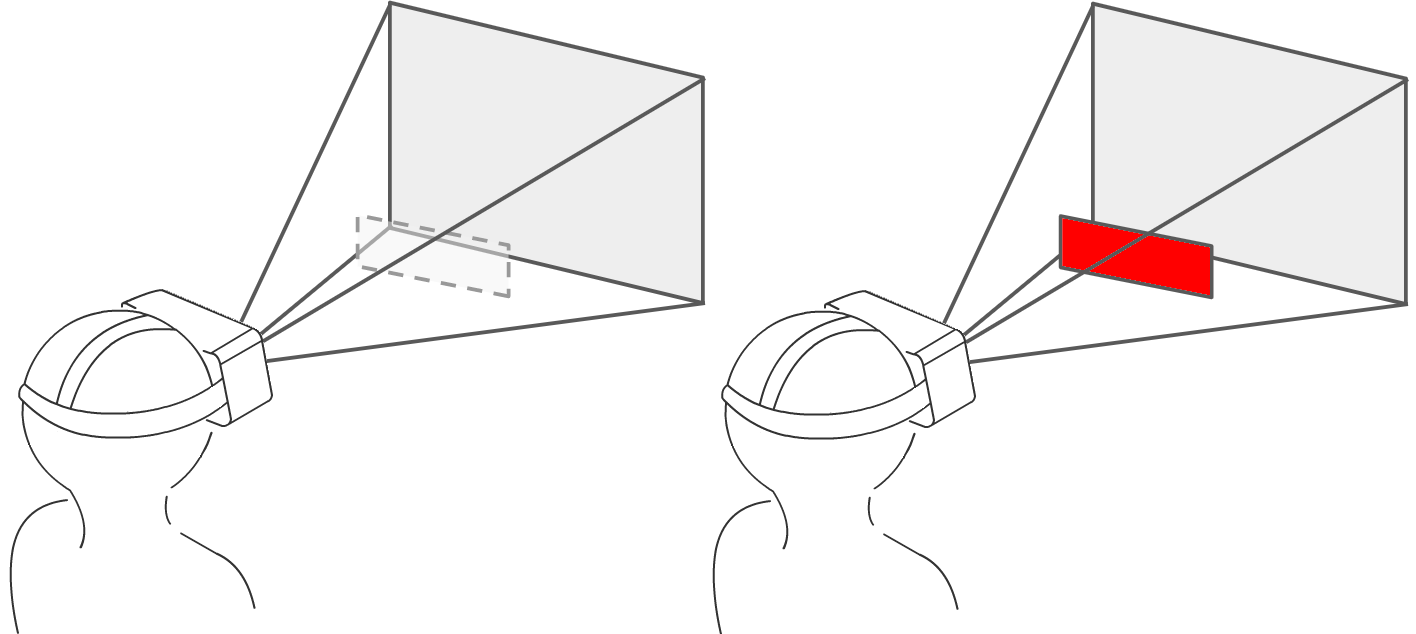
\includegraphics[width=0.75\textwidth]{imagenes/7/camera-overlay.png}
\caption{Cuadro de texto superpuesto al mundo}
\label{fig:camera-overlay}
\end{center}
\end{figure}

Además, Unity trabaja por defecto con letras rasterizadas; es decir, pueden verse muy fácilmente sus píxeles. Esto, aunque el texturas no es tan importante, hace que sea difícil leer texto, y más aún con unas gafas de realidad virtual. Por tanto, y tras investigar, se decidió utilizar la librería de Unity \textbf{TextMeshPro} que proporciona soporte para letras vectoriales, lo que hace que da igual a la distancia o el tamaño al que se rendericen que aparecerán extremadamente nítidas. Como único inconveniente, es necesario convertir las fuentes que se estén utilizando en el proyecto a su formato propio, aunque la propia librería proporciona una herramienta para poder hacerlo cómodamente.

Por tanto, una vez que se disponía de letras legibles que seguían al jugador fue momento de hacer que el cuadro apareciera con la descripción de un cuadro (cargada desde un archivo de texto en disco) cuando el jugador estuviera cerca de él y pulsara un botón.

Para ello, cada cuadro tiene un script llamado \texttt{PaintingDescription-} \texttt{Manager.cs}, que utiliza una esfera de colisión para detectar cuándo se encuentra cerca el jugador y, cuando lo hace, activa un pequeño icono enfrente del jugador para que éste sepa que tiene disponible la descripción de un cuadro pulsando un botón.

A continuación, cuando el jugador pulsa el botón el script se encarga de escribir su descripción, que previamente ha leído de disco, en el cuadro delante del jugador, y después lo vuelve visible para que pueda ser leído. Este cuadro vuelve a ser invisible tanto si el jugador deja de pulsar el botón como si se aleja del cuadro.

Este script necesita la sala en la que se encuentra y el nombre del cuadro, para poder encontrar el directorio con el archivo que tiene que leer, las referencias a ambos mandos, para saber cuándo se pulsa y libera el botón correspondiente, y las referencias al cuadro, al icono de disponibilidad y al objeto TextMeshPro para poder escribir en él. De este modo se consigue que el jugador solo tenga un cuadro de texto, que es accedido por todos los cuadros y modificarlo.

En el listado \ref{lst:painting-description} puede verse el fragmento de código de este script encargado de detectar si el jugador está cerca y activar el icono de disponibilidad y, si además pulsa el botón adecuado, activará el cuadro de texto y escribirá en él su descripción.

\begin{lstlisting}[caption=Fragmento del script para activar la descripción de los cuadros, label=lst:painting-description]
private void OnTriggerEnter(Collider other)
{
    if (other.name.Contains(PLAYER_TAG))
    {
        playerIsNear = true;
        availabilityIcon.SetActive(true);
    }
}
    
private void ControllerEvents_ButtonTwoPressed(object sender, ControllerInteractionEventArgs e)
{
    if (playerIsNear)
    {
        textObject.text = paintingDescription;
        availabilityIcon.SetActive(false);
        textBackground.SetActive(true);
        PlaySoundEffect();
    }
}
\end{lstlisting}

Además, en las últimas líneas puede leerse cómo se llama al método encargado de reproducir un pequeño efecto de sonido, que sería implementado en una de las últimas entregas.

\subsection{Fundido a negro entre salas}

Además, como otro de los objetivos de esta entrega era realizar un fundido a negro al cambiar de salas, se utilizó un plano negro colocado frente a la cámara de manera similar que el de la descripción de los cuadros, aunque más cerca. Este plano comienza la escena completamente opaco y ve reducido su opacidad gradualmente hasta ser completamente transparente, lo que da al jugador el efecto de un fundido desde negro. Como vuelve a ser necesario realizar la interpolación lineal de un parámetro entre dos valores a lo largo del tiempo, como en la entrega anterior, se utilizó la función \texttt{Lerp} de la clase \texttt{Color} para actualizar el color del plano.

\subsection{Prototipado de un arco}

Para finalizar esta entrega, la última tarea que falta es desarrollar el prototipo de un sistema de interacción avanzado que se finalizaría y perfilaría en la siguiente entrega. La idea era implementar un sistema que permitiera al jugador disparar y aunque se valoraron varios tipos, como pistolas, finalmente se decidió que el más interactivo para el jugador, además de el que más cuadraba con las temáticas del museo, sería un arco.

Para ello se utilizaron diversos componentes genéricos del framework \acs{VRTK}, además de otros desarrollados específicamente para arcos, como animaciones de tensado o un script que permitía apuntar, \texttt{BowAim.cs}. Además, el modelo del arco, que también provee la librería, se adaptó para coincidir con la estética del juego.

Tras ello, se modeló un carcaj y una flecha y se utilizó el script \texttt{Arrow-} \texttt{Spawner.cs} para hacer que el jugador pudiera sacar flechas infinitamente del mismo. Finalmente, se desarrolló un script que permitía detectar las colisiones de las flechas con objetos.

Por lo tanto, el resultado de esta entrega fue una versión del proyecto con todas las salas completas hasta el barroco, que sería la siguiente, y un prototipo funcional de un arco listo para ser utilizado. Además, el usuario puede consultar la descripción de los cuadros y hay un fundido a negro al cambiar de escena, aparte de otras características menores. En el vídeo que se presenta a continuación pueden verse estos avances.

\begin{center}
    \url{https://youtu.be/MLn0r248dUs}
\end{center}



\section{Entrega 4}

Una vez que se disponía del prototipo funcional de un arco capaz de disparar flechas, se comenzó a modelar la siguiente sala cuyo boceto, dibujado antes de comenzar para disponer de un punto de partida, puede verse en la figura \ref{fig:boceto-sala-4}

\begin{figure}[!h]
\begin{center}
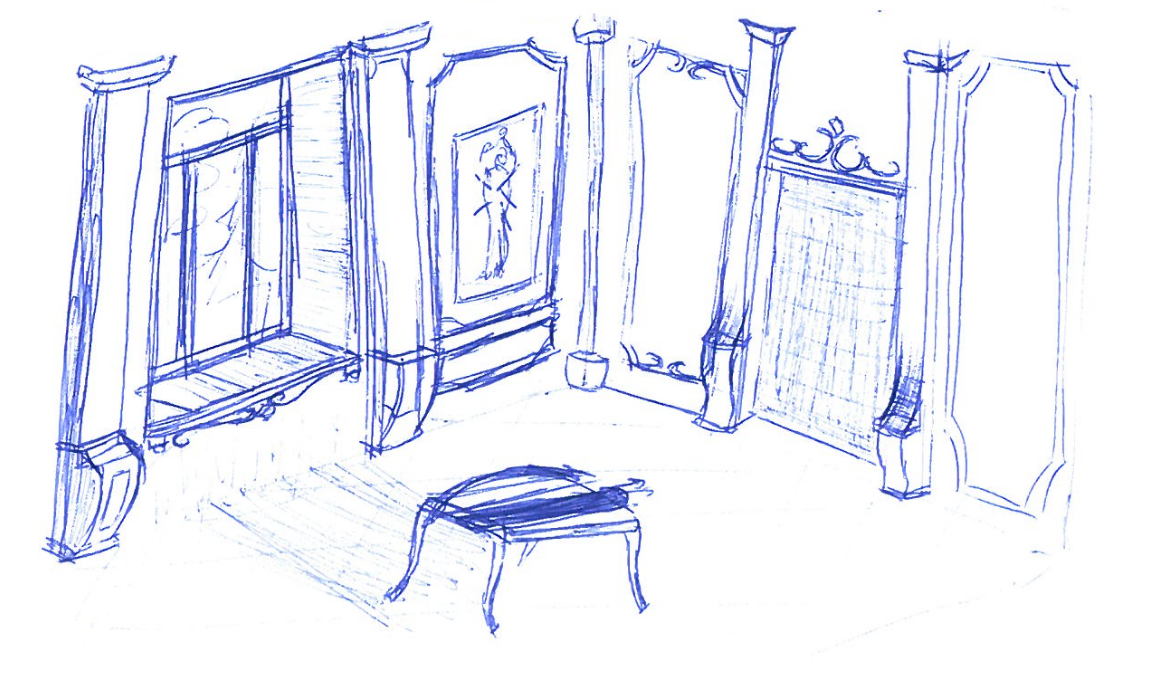
\includegraphics[width=0.75\textwidth]{imagenes/7/bocetos/boceto-sala-4.png}
\caption{Boceto de la cuarta sala}
\label{fig:boceto-sala-4}
\end{center}
\end{figure}

En este boceto se propuso colocar una mesa en el centro con el arco y el carcaj encima. De este modo, sería fácil para el jugador visualizar todos los objetivos que hubiera en la sala y dispararles. Además, también pueden verse grandes ventanas que permiten que entre más luz. Aunque en el boceto no se ve, porque aún no se tenía claro, finalmente el techo también fue abierto, como puede verse en el la figura \ref{fig:unity-sala-4}.

\subsection{Limitando el peso por texturas}

Por otro lado, al comienzo del modelado de esta sala se empezó a ver que el espacio dedicado a las texturas era cada vez más y más grande. Inicialmente, para cada textura de Unity se utilizaban todos los mapas descargados, y la mayoría de ellos llegaba a una resolución de 4K, llegando a pesar cada uno varios megas, cuando no era necesaria para nada tanta resolución. Por ello, y tras comprobar que se veían bien, se decidió reducir todas las texturas a 1024\texttt{x}1024 píxeles y trabajar para cada textura únicamente con 3 mapas diferentes, que han sigo los siguientes.

\begin{itemize}
    \item Un mapa de color, que sería la textura propiamente dicha. En Unity, este mapa se llama \textbf{albedo}, que en física es el porcentaje de radiación que refleja una superficie respecto a la que incide sobre ella.
    \item Un mapa de normales, que proporciona relieve al modelo y ayuda a evitar que se vea plano, dándole realismo.
    \item Un mapa de oclusión, que define cómo reflejará la luz cada parte del modelo. Eso se vuelve especialmente útil en texturas con varios materiales (como metal y ladrillo), haciendo que no se vean iguales.
\end{itemize}

Por ello, se decidió repetir la textura del suelo de la primera sala en esta, de nuevo, al comprobar que casaba relativamente bien con el color de las paredes. La versión final de esta sala, con los cuadros colocados, puede verse en la figura \ref{fig:unity-sala-4}.

\begin{figure}[!h]
\begin{center}
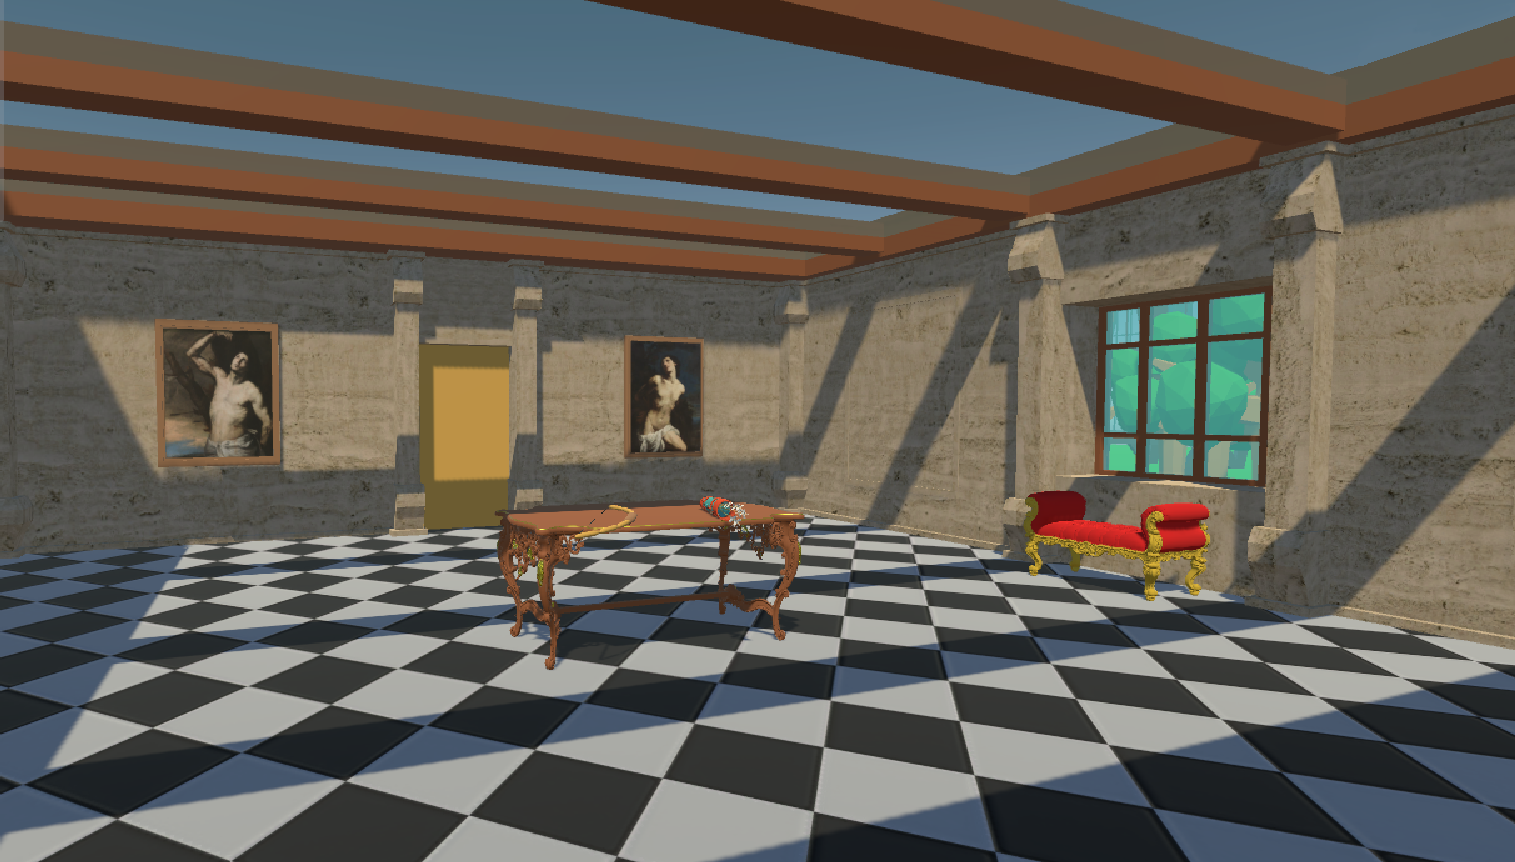
\includegraphics[width=0.85\textwidth]{imagenes/7/salas-unity/unity-sala-4.png}
\caption{Sala 4 renderizada en Unity}
\label{fig:unity-sala-4}
\end{center}
\end{figure}

\subsection{Disparando a los cuadros}

Tras esto, se importó el arco desde la escena de prueba hasta la definitiva y se comenzó a trabajar en un sistema capaz de informar al usuario a qué cuadro debe disparar de manera orgánica y detectar sus disparos. Finalmente se ha implementado un sistema que hace brillar parpadeando el borde del cuadro que el jugador tiene que disparar y lo ilumina en verde cuando acierta con una flecha para luego volver a su color original. Finalmente, cuando todos los cuadros han sido acertados las veces necesarias y el juego ha terminado, todos comienzan a parpadear con luz amarilla durante unos segundos y luego vuelven a la normalidad.

Para dividir el trabajo entre varios scripts, se ha diseñado el siguiente sistema. Por un lado, cada cuadro tiene un script, \texttt{PaintingCollider-} \texttt{Detector.cs}, que le permite definir todos los parámetros necesarios para cada cuadro, como el material al que tienen que cambiar, el tiempo de fundido, si están activos o no... que se comunican con un gestor global, \texttt{ArrowGameManager.cs}, que elije qué cuadro será objetivo, y al que informan cuando un cuadro activo se acierta para que pueda llevar la cuenta de la puntuación, y finalmente activar la luz de victoria en todos los cuadros y desbloquear la puerta. En entregas futuras este script también activaría determinados diálogos del vigilante. Además, para evitar que los cuadros estuvieran brillando cuando el jugador entrara a la sala y antes de haber tenido tiempo de hablar con el vigilante para que le explique el juego, se ha hecho que el gestor del juego sea notificado cuando el jugador toque el arco para empezar, lo que se ha conseguido con el script \texttt{BowInformer.cs}, que utiliza una esfera de colisión en el mango para saber cuándo el jugador lo está sosteniendo. Además, el arco también contiene el script para teletransportarse de vuelta a la mesa si toca el suelo.

A continuación, la figura \ref{fig:sequence-diagram-bow} contiene el diagrama de secuencia que intenta presentar de un modo más visual lo que se ha explicado anteriormente. Aunque en Unity la vida de un objeto es más amplia, ya que se inician cuando la escena comienza y se destruyen cuando acaba, se ha adaptado para representar mejor cuándo interviene cada clase.

\begin{figure}[!h]
\begin{center}
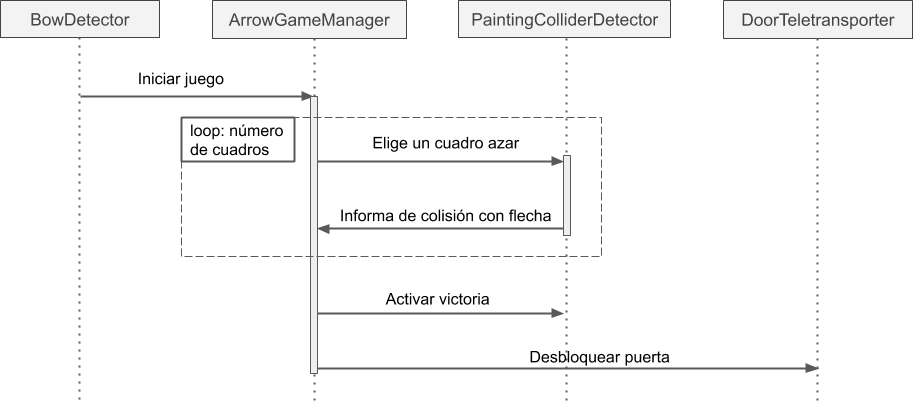
\includegraphics[width=1\textwidth]{imagenes/7/bow-sequence-diagram.png}
\caption{Diagrama de secuencia del juego del arco}
\label{fig:sequence-diagram-bow}
\end{center}
\end{figure}

Para gestionar el estado de un cuadro, que puede ser \texttt{Disabled}, \texttt{Enabled}, \texttt{FadingToDisabled} y \texttt{Winning}, se ha utilizado un \texttt{switch} dentro del método \texttt{Update()} que comprueba en cada frame su estado y actúa en consecuencia. Para cambiar su material, de nuevo, se ha utilizado la función \texttt{Lerp} de interpolación lineal. 
En el listado \ref{lst:painting-collider} puede verse cómo funciona el \texttt{switch} mencionado anteriormente, cambiando su comportamiento dependiendo del estado, que actualiza de forma asíncrona el gestor del juego, y cómo se informa al gestor del juego cuando una flecha colisiona con un cuadro cuando éste está activo.

\begin{lstlisting}[caption=Fragmento del script para actualizar un cuadro, label=lst:painting-collider]
private void Update()
{
    switch (state)
    {
        case PaintingState.Disabled:
            break;
        
        case PaintingState.Enabled:
            pingpong = Mathf.PingPong(Time.time, 
                                      FadingInDuration);
            fadingLerp =  pingpong / FadingInDuration;
            GetComponent<Renderer>().materials[1].Lerp(
                                        LightMaterial,
                                        FrameMaterial,
                                        fadingLerp);
            break;
    
        case PaintingState.Winning:
            ...
    }
}

private void OnTriggerEnter(Collider other)
{
    if (state != PaintingState.Disabled && 
        other.tag == ARROW_TAG)
    {
        gameManagerScript.
            AnnounceDetectedArrow(this.name);
    }
}
\end{lstlisting}

Como puede verse, al colisionar con un objeto que resulta ser una flecha se anuncia al gestor del juego lo ocurrido para que se encargue de ello. En el listado \ref{lst:painting-manager} puede verse este método y cómo comprueba cuántos cuadros se han acertado y si quedan más. De ser así, elige un cuadro aleatoriamente (que no puede ser el mismo) y le hace saber que es el elegido; por el contrario, si el juego ha terminado, lo anuncia a todos los cuadros para que ellos lo gestionen y parpadeen en amarillo durante unos instantes.

\begin{lstlisting}[caption=Fragmento del script para gestionar el juego del arco, label=lst:painting-manager]
public void AnnounceDetectedArrow(string painting_name)
{
    painting_scripts[currentIndex].Disable();
    successfulShots++;

    if (successfulShots >= MaxShoots)
    {
        foreach (PaintingColliderDetector pcd
                    in painting_scripts)
        {
            pcd.Win();
        }
    }
    else
    {
        currentIndex = GenerateNewIndex();
        painting_scripts[currentIndex].Enable();
    }
}
\end{lstlisting}

\subsection{Mostrando un candado en las puertas bloqueadas}

Por otro lado, al empezar a probar el proyecto con jugadores reales se vio que no había ningún tipo de retroalimentación en el momento en el que la puerta se desbloqueaba; es decir, el jugador no sabía cuando podía pasar a la siguiente sala ni qué puertas estaban bloqueadas. Por ello, se colocó la imagen de un candado delante de las puertas bloqueadas que, gestionado por el propio script que activa y desactiva el teletransporte, es visible cuando el jugador no puede utilizarla y es deshabilitado y desaparece cuando la puerta es usable.

Por último, antes de pasar a la siguiente entrega, se comenzó a trabajar en la siguiente sala, la quinta, ambientada en el romanticismo. Como tal, se intentó dar un aspecto místico utilizando poca luz y un sistema de partículas de niebla, aunque éste no fue implementado hasta la siguiente entrega.

Como tanto la cuarta sala, con el arco y las flechas, como la sexta, que previsiblemente implementaría un juego de piezas de cuadros en forma de puzzle, se consideraban bastante activas, se decidió diseñar la quinta para que fuera más tranquila y el jugador pudiera relajarse. Por tanto, se pensó en esconder la llave para desbloquear la puerta de salida en los cajones de un mueble y colocar varios cuadros con pistas escondidas que llevaran al jugador hasta la llave, obligándole así a examinarlos con detalle.

Así, el boceto generado para esta sala puede verse en la figura \ref{fig:boceto-sala-5}, que contiene el mueble con los cajones (y un par de sillas para no hacerlo tan evidente), una alfombra que finalmente se eliminó y unas gruesas cortinas que tapan la luz del exterior.

\begin{figure}[!h]
\begin{center}
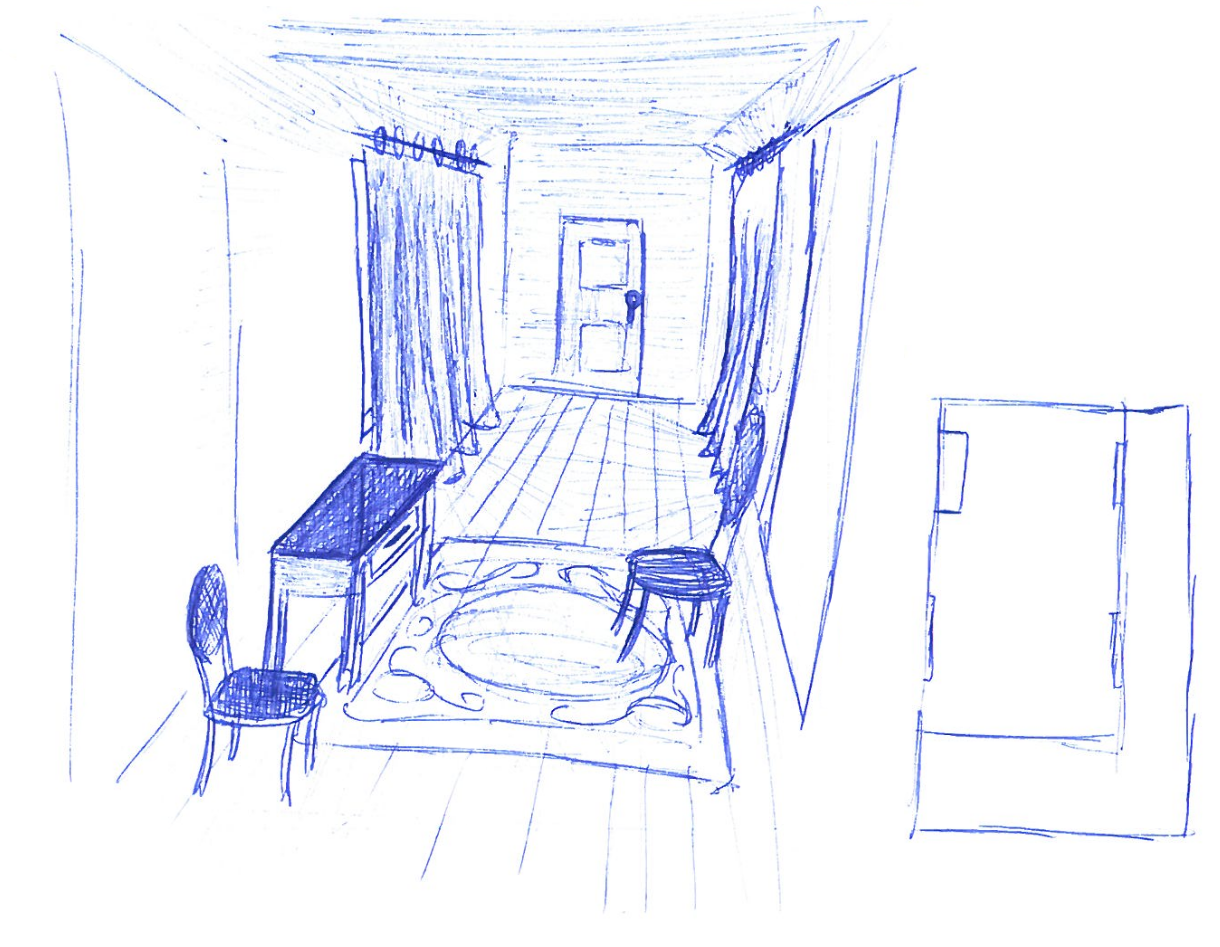
\includegraphics[width=0.75\textwidth]{imagenes/7/bocetos/boceto-sala-5.png}
\caption{Boceto de la quinta sala}
\label{fig:boceto-sala-5}
\end{center}
\end{figure}

Pero apenas se comenzó a modelarla cuando llegó la fecha de finalización de la entrega, por lo que se terminó de trabajar en la misma y se grabó el vídeo mostrando el resultado hasta la fecha, que incluía las cuatro primeras salas terminadas y pequeños añadidos como los candados de las puerta. Dicho vídeo puede verse a continuación.

\begin{center}
    \url{https://youtu.be/w83YTZuz6tQ}
\end{center}



\section{Entrega 5}

Tras dar por finalizada la entrega 4, la primera tarea en la que comenzó a trabajar fue el terminar el modelado de la quinta sala. Como ya se ha comentado antes, finalmente la alfombra de en medio se eliminó y fue sustituida por la estatua de \textit{El pensador}, además de situar los cajones al fondo para intentar ocultarlos. 

\subsection{Niebla virtual}

Para generar niebla realista se han utilizado dos componentes simultáneamente. Por un lado, se ha utilizado un sistema de partículas  que, a partir de un \textit{tileset} o conjunto de imágenes de humo, consigue generar imágenes translúcidas y en movimiento a lo largo de la sala. Además, se ha configurado este sistema para que roten y cambien de dirección ligera y aleatoriamente, dando la sensación de bruma cambiante. 

Por otro, se ha utilizado el sistema de iluminado para simular lo que se conoce como \textit{deferred fog}\footnote{\url{https://docs.unity3d.com/Manual/PostProcessing-Fog.html}} o niebla diferida. Este efecto superpone un color a los objetos dependiendo de lo lejos que estén de la cámara; así, si un objeto está cerca se verá tal cual pero si se aleja se irá volviendo poco a poco del color indicado. En este caso el color elegido has sido gris, lo que junto al sistema de partículas simula de un modo lo suficientemente realista el efecto óptico que genera la niebla real.

El resultado final de esta sala puede verse en la figura \ref{fig:unity-sala-5}.

\begin{figure}[!h]
\begin{center}
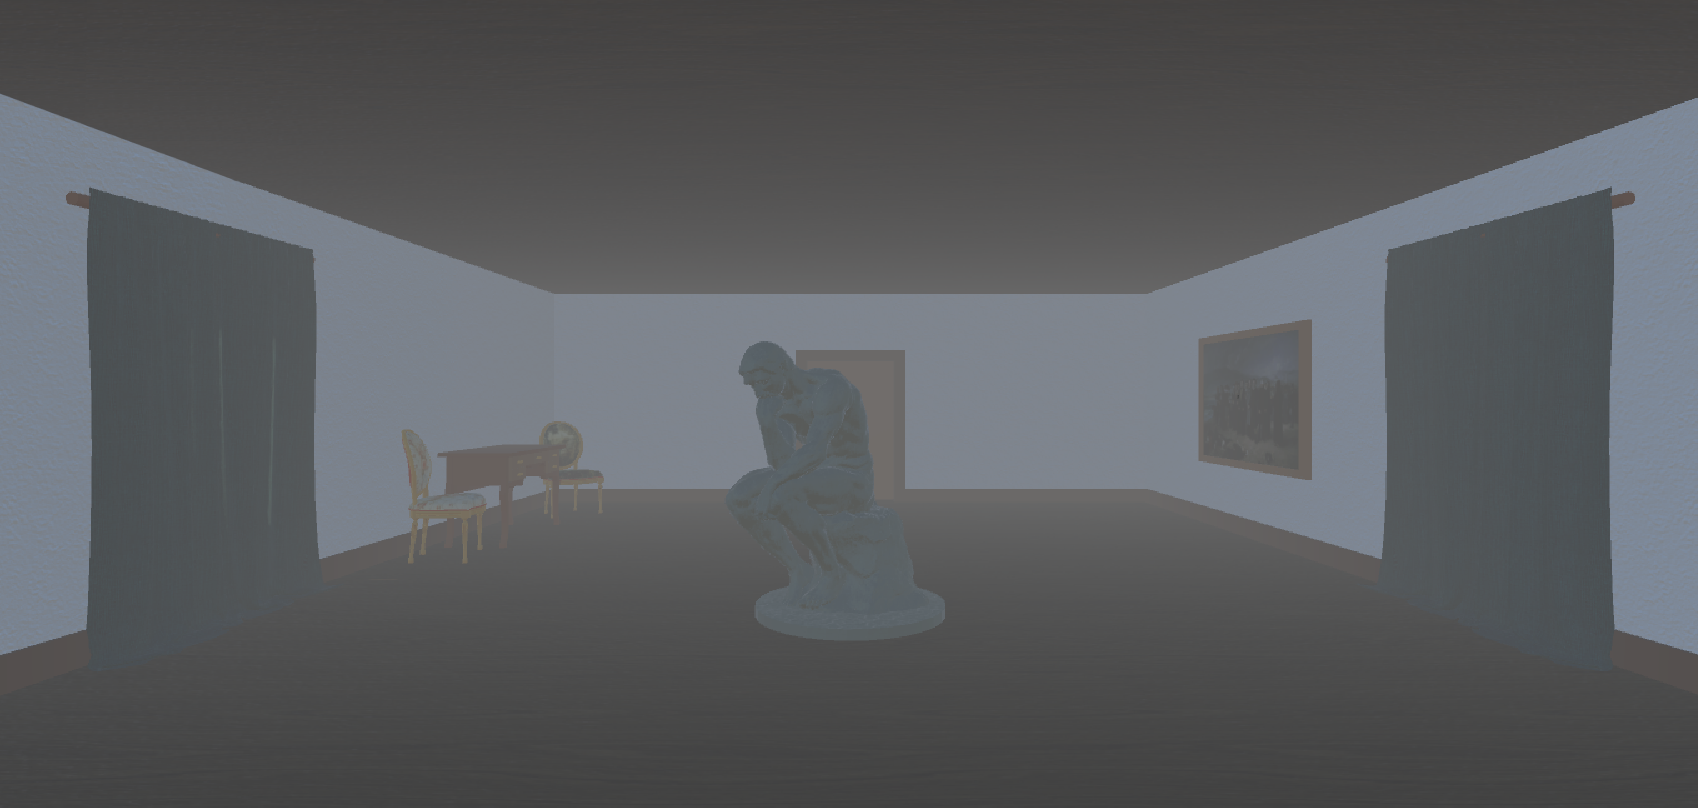
\includegraphics[width=0.85\textwidth]{imagenes/7/salas-unity/unity-sala-5.png}
\caption{Sala 5 renderizada en Unity}
\label{fig:unity-sala-5}
\end{center}
\end{figure}

\subsection{Cuadros con pistas y cajones interactivos}

Una vez que la sala estaba terminada se pasó a implementar el acertijo elegido. Como ya se introdujo anteriormente, la quisicosa para esta sala sería un cajón interactivo escondiendo la llave de la puerta de salida y las sílabas de la palabra \textit{cajones} en cada uno. Por ello, en cada uno de los 3 de la sala se colocó un cuadro de texto con la librería TextMeshPro para que pudieran leerse siempre nítidamente. El cuadro \textit{Doña Juana la Loca} contiene la sílaba \textit{CA} cerca del ataúd de Felipe el Hermoso, el cuadro \textit{El caminante sobre un mar de nubes} contiene la sílaba \textit{JO} entre la niebla y por último el cuadro \textit{El Fusilamiento de Torrijos y sus compañeros} contiene la sílaba \textit{NES} cerca del general. Además, cada uno de los textos tiene un color muy parecido a la parte que sobre la que están colocados.

Para terminar con esta sala, se procedió a implementar los cajones interactivos. Para ello, tras modelar una pequeña mesa con cinco cajones y una llave antigua en Blender, se importaron a Unity y se utilizó el script \texttt{VRTK\_Physics\_Slider.cs} para hacer que los cajones se pudieran deslizar en una dirección y se colocó la llave dentro de uno de ellos. El problema con este script fue que lo que en teoría debería haber sido algo relativamente directo se convirtió en un interminable ajuste de parámetros para conseguir que el sistema funcionara correctamente, e incluso fue necesario bucear en el código fuente del framework para averiguar por qué no lo hacía. Finalmente fue necesario escribir un pequeño script, llamado \texttt{CollisionIgnorer.cs}, para hacer que la llave ignorara la caja de colisión con la mesa. Como puede verse en el listado \ref{lst:collision-ignorer}, este script hace uso de la interfaz al motor de físicas de Unity y comprueba cuando colisiona con un objeto si corresponde con el que se ha indicado que ignore para indicarle que lo haga.

\begin{lstlisting}[caption=Fragmento del script para ignorar colisiones, label=lst:collision-ignorer]
public GameObject ignoredObject;

 void OnCollisionEnter(Collision collision)
{
    if (collision.gameObject.name == ignoredObject.name)
    {
        Physics.IgnoreCollision(
                    collision.collider, 
                    GetComponent<Collider>());
    }
}
\end{lstlisting}

Por último, para hacer que el jugador pudiese colocar la llave en la cerradura de la puerta, que no era más que una imagen como se explica en la entrega anterior, se utilizó una \textit{snap drop zone} estratégicamente colocada en el ojo de la cerradura para que pareciese que realmente estaba activando su mecanismo, y como ya se ha explicado anteriormente su uso esta vez se omitirá. Por último, para detectar cuando la llave es colocada se utiliza el script \texttt{KeyDetector.cs} que se suscribe al evento que emite la clase \texttt{VRTK\_SnapDropZone} cuando se le coloca un objeto, comprueba que se trata de la llave y de ser así se lo comunica al script de la puerta, que oculta el candado y se activa para permitir al usuario pasar a la siguiente sala.

\subsection{Descripción de la sala de las vanguardias}

Así, una vez que se terminó la quinta sala, se comenzó a trabajar en la sexta y, como en el resto, se comenzó por su boceto, que puede verse en la figura \ref{fig:boceto-sala-6}. Como se ha introducido anteriormente, en esta sala hay cuatro cuadros, divididos en cuatro piezas cada uno, que el jugador tiene que colocar en su sitio y en orden. En cada pared, además del hueco para las piezas y una pequeña miniatura del cuadro que el jugador puede usar como referencia, hay una bombilla que indica mediante su color si el cuadro está sin terminar, brillando en amarillo, si el cuadro se ha terminado pero mal, brillando en rojo, y si el cuadro es correcto, con lo que brillaría en verde. El utilizar una bombilla que cambie de color es la interfaz más natural con el jugador y la manera más orgánica de proporcionarle retroalimentación que se ha valorado.

\begin{figure}[!h]
\begin{center}
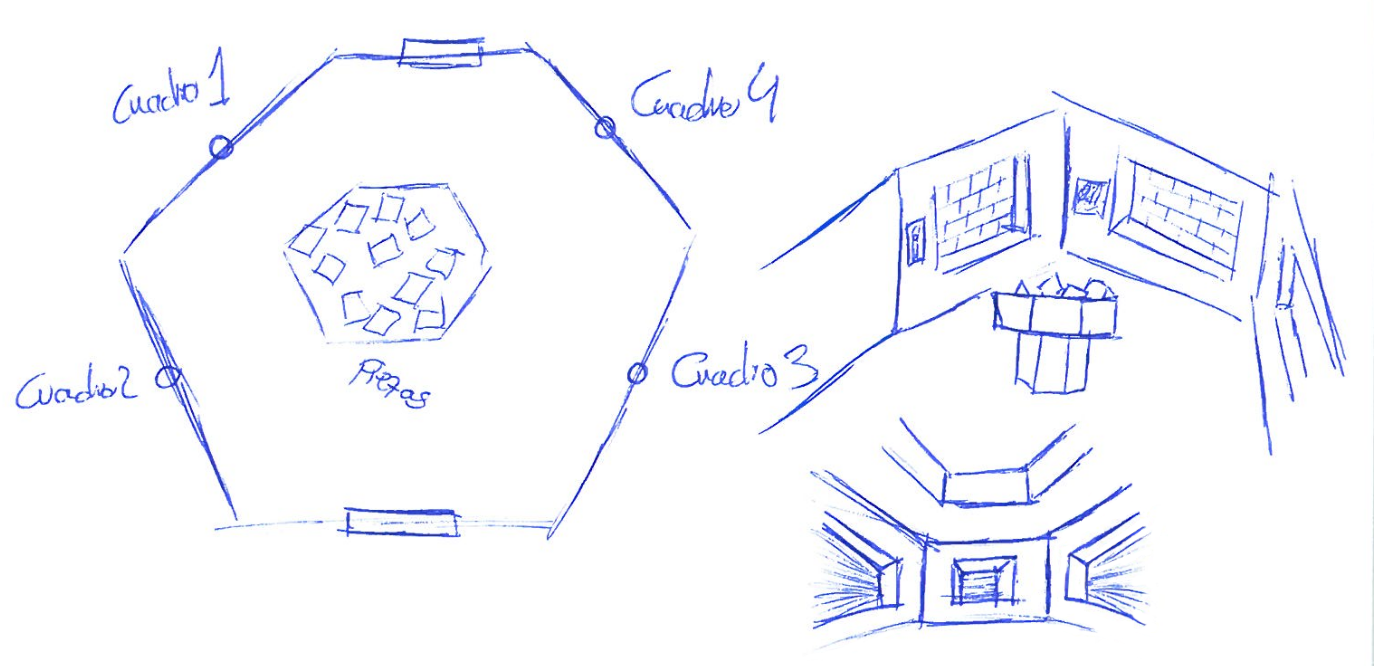
\includegraphics[width=0.75\textwidth]{imagenes/7/bocetos/boceto-sala-6.png}
\caption{Boceto de la sexta sala}
\label{fig:boceto-sala-6}
\end{center}
\end{figure}

Como está ambientada en las vanguardias del siglo XX, se ha intentado dar un aspecto más modernista a esta sala modelándola con amplias paredes blancas con forma hexagonal, lo que coincide con el tener cuatro cuadros, uno en cada pared, más dos para las puertas de entrada y salida. Además, también se ha utilizado una textura de azulejos con forma pseudo-hexagonal para el suelo. 

Por otro lado, en el centro de la sala se encuentra un pequeño recipiente con las 12 piezas de los cuadros que el jugador debe coger para colocarlas.

Finalmente, encima de la puerta de salida que, como indica el guardia, lleva a su almacén (en el que es finalmente desenmascarado como el ladrón de guante blanco), se ja colocado un pequeño letrero en el que puede leerse \textit{Staff}.

La imagen con la versión final de la sala puede verse en la figura \ref{fig:unity-sala-6} con todos los elementos explicados anteriormente. Aunque en el juego evidentemente las piezas no pueden aparecer puestas y en el contenedor del centro, en la imagen se muestran ambas para que el lector pueda hacerse una idea de cómo quedan tanto colocadas como antes de hacerlo.

\begin{figure}[!h]
\begin{center}
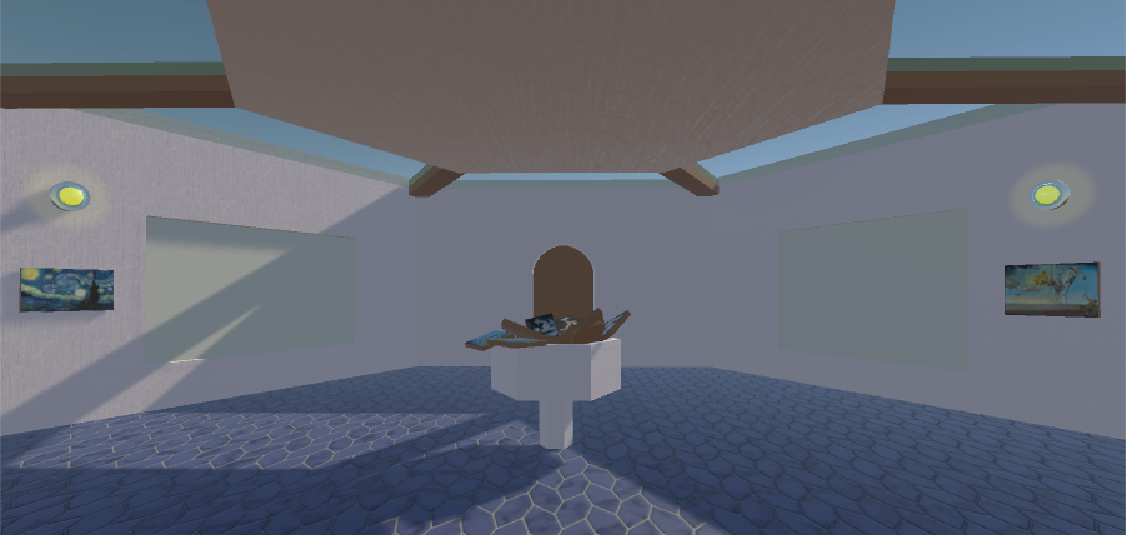
\includegraphics[width=0.85\textwidth]{imagenes/7/salas-unity/unity-sala-6.png}
\caption{Sala 6 renderizada en Unity}
\label{fig:unity-sala-6}
\end{center}
\end{figure}

\subsection{Puzzles virtuales con piezas de cuadros}

Una vez explicado el modelado de la sala, se pasará a contar cómo se ha implementado el sistema de puzzles con las piezas. Lo primero que es necesario contar es que, al igual que en todos los casos anteriores en los que se requería que el usuario colocase objetos en lugares específicos, se ha usado la combinación de objetos interactivos (en este caso las piezas de los cuadros) con \textit{snap drop zones} (los huecos en los que es necesario colocarlos).

Para implementar este sistema se ha utilizado un diseño \textit{master/slave} parecido al del arco que dispara a cuadros, en el que hay un çunico componente con una idea global de lo que está pasando encargado de controlar al resto, que simplemente le informan de lo que pasa y actúan cuando se lo ordena.

En este caso, los \textit{slaves} son las cuatro instancias del script \texttt{Painting-} \texttt{Checker.cs}, una por cada cuadro. Este script es el encargado de manejar las cuatro \textit{snap drop zones} de las que se compone un cuadro (una para cada pieza), detectando cuándo se coloca y se retira una pieza. Además, como la nomenclatura que se ha seguido para las piezas y las zonas ha sido llamar a cada zona con el mismo nombre que la pieza que tiene que contener, es sencillo para el script saber si ésta está en su lugar o no.

Para este puzzle ha sido de vital importancia colocar las zonas justo donde corresponden, para que cuando el cuadro esté completado no se noten los cortes entre ellas. Esta tarea ha sido relativamente compleja y ha sido necesario apuntar manualmente las posiciones exactas desde Blender y hacer el cálculo de cambio de ejes a Unity, ya que los ejes \texttt{X}, \texttt{Y}, \texttt{Z} en Blender corresponden a \texttt{X}, \texttt{Z}, \texttt{-Y} en Unity.

En la figura \ref{fig:painting-piece-hover} puede verse cómo se ilumina una zona al pasar el cuadro por encima, que por defecto es invisible; de este modo es posible para el jugador saber en qué sitio está colocando la pieza.

\begin{figure}[!h]
\begin{center}
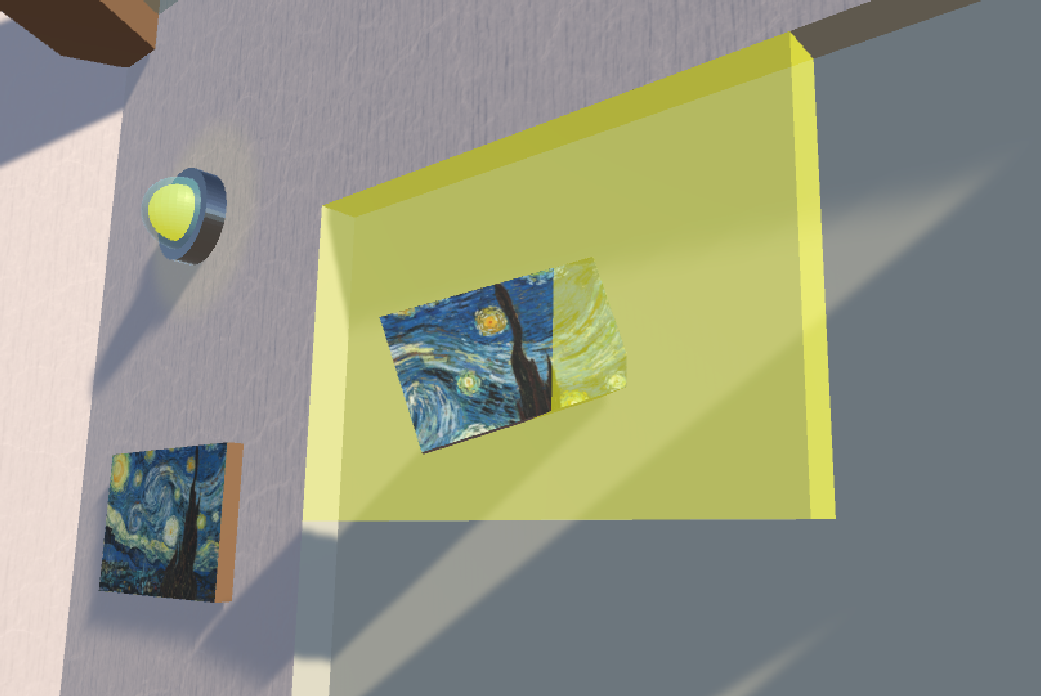
\includegraphics[width=0.5\textwidth]{imagenes/7/painting-piece-hover.png}
\caption{Pieza de un cuadro sobre uno de los posibles huecos}
\label{fig:painting-piece-hover}
\end{center}
\vspace{-0.5cm}
\end{figure}

Como puede verse, la pieza es tres veces menor que la zona, y una vez puesta triplicará su tamaño. Esto se ha hecho así porque al principio del diseño se vio que las piezas del cuadro eran demasiado grandes para ser manejadas con comodidad, lo que no era posible hasta que medían aproximadamente un tercio de su tamaño. Así, se ha configurado la zona para que al colocar un objeto sobre ella que sea del tipo esperado haga aumentar su tamaño tres veces.

Para poder detectar cuándo se colocan objetos, el script suscribe el mismo método al evento de todas sus zonas que informan de éste hecho. Aunque se podría haber suscrito un método a cada uno y se sabría de antemano qué zona es la que lo ha emitido, este diseño es mucho más compacto y reutilizable e implica menos duplicidad de código.

A continuación, en el listado \ref{lst:painting-checker} puede verse cómo cuando se coloca una pieza en una de las cuatro \textit{snap drop zones} que gestiona cada script se llama al siguiente método, que compruba, primero, que el cuadro no esté ya terminado. Si no lo está, aumenta en uno el número de piezas que tiene y, si la pieza ha sido colocada en su sitio, aumenta en uno el número de piezas correctas, pero si no y si está lleno enciende la luz roja. Por el contrario, si todas las piezas han sido colocadas correctamente el cuadro ha sido terminado, por lo que cambia la bombilla a verde, deshabilita las cajas de colisión de todas las piezas para que puedan ser retiradas e informa al \textit{master} de que el cuadro ha sido terminado correctamente.

\begin{lstlisting}[caption=Fragmento del script detectar piezas de cuadros, label=lst:painting-checker]
internal void OnPieceSnapped(object sender, 
                        SnapDropZoneEventArgs e)
{
    if (!isCorrectlyFinished)
    {
        currentPieces++;
    
        string objectName = e.snappedObject.name;
        string zoneName = sender.ToString();
    
        if (PieceIsCorrect(objectName, zoneName))
        {
            correctPieces++;
            if (correctPieces == MAX_PIECES)
            {
                isCorrectlyFinished = true;
    
                ChangeBulbColor(LightGreen);
                LockAllPiecesInPlace();
    
                gameManagerScript.PaintingFinished();
            }
        }
    
        if (currentPieces == MAX_PIECES 
            && !isCorrectlyFinished)
        {
            ChangeBulbColor(LightRed);
        }
    }
}
\end{lstlisting}

Por otro lado, el \textit{master} del sistema es el script \texttt{PaintingPiecesGame-} \texttt{Manager.cs}. Este componente es informado de los eventos que suceden y actúa en consecuencia. Además, de manera similar a la sala del arco, cuando el jugador entra en esta sala todas las bombillas están apagadas, y no se encienden hasta que el jugador se acerca al contenedor central. Este recipiente tiene un script, \texttt{GameStarter.cs}, que informa al \textit{master}, quien a su vez le indica a todos los \textit{slaves} que enciendan las luces. Finalmente, cuando ha recibido un número de mensajes igual al tamaño de su vector de \textit{slaves} desbloquea la puerta de salida para que el jugador pueda continuar.

En entregas posteriores se integraría el gestor de diálogos del vigilante para que hablara cada vez que un cuadro era completado.

Finalmente, antes de terminar la entrega se grabó un vídeo demostrativo, explicando todos los cambios implementados a lo largo de la misma, que puede verse en el siguiente enlace.

\begin{center}
    \url{https://youtu.be/WDkoSrzh24o}
\end{center}



\section{Entrega 6}

Lo primero que se comenzó a hacer en la entrega 6 fue modelar la séptima sala, el almacén del vigilante, en la que el juego llega a su desenlace y se desenmascara finalmente al ladrón del cuadro.

\subsection{El almacén del vigilante y el cuadro robado}

Para esta sala, como en comparación con el resto es más simple, no fue necesario realizar un boceto y se pasó directamente a modelarla. Es una habitación cuadrara, relativamente pequeña, para la que se ha utilizado una textura de pintura desconchada para las paredes y de cemento para el suelo para que, en contraposición con el resto del museo, parezca vieja y abandonada, en un intento de destapar al vigilante alguien malvado. Además de las estanterías, la sala cuenta con varias cajas y palés, algo que temáticamente encajaría en un almacén, que puede verse terminada en la figura \ref{fig:unity-sala-7}.

\begin{figure}[!h]
\begin{center}
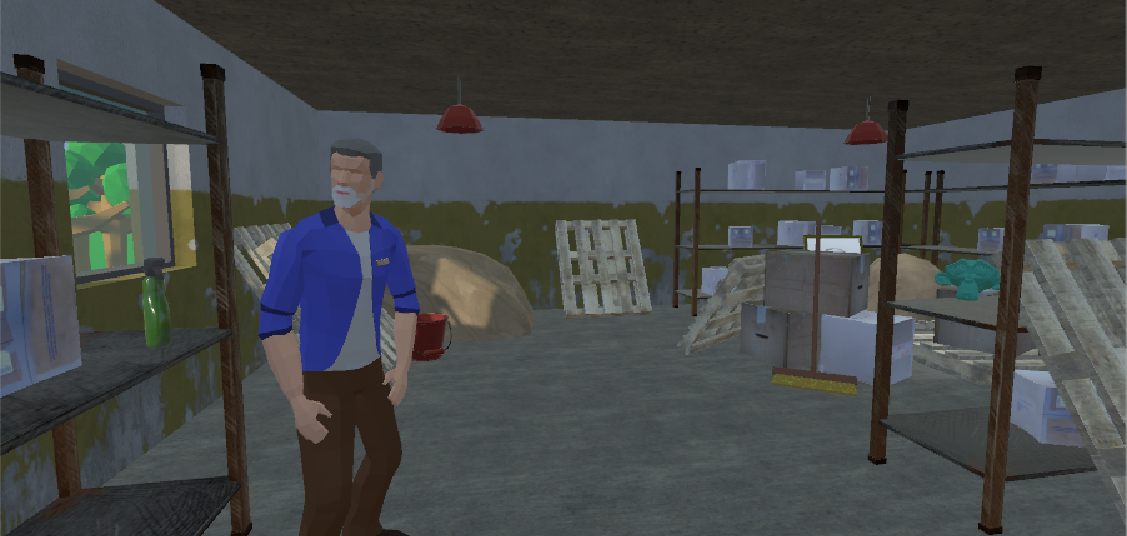
\includegraphics[width=0.85\textwidth]{imagenes/7/salas-unity/unity-sala-7.png}
\caption{Sala 7 renderizada en Unity}
\label{fig:unity-sala-7}
\end{center}
\vspace{-0.35cm}
\end{figure}

Además, para dar más realismo a la sala, se han colocado diversos objetos temáticos, como cubos, un limpiacristales o Suzanne, el icónico logo de Blender con forma de cabeza de mono. Además, el jugador puede interactuar con todos ellos.

En el centro de la sala, encima de una silla y tapado por diversos objetos como cajas y cepillos que el jugador tendrá que quitar de en medio para llegar hasta él, se encuentra el cuadro robado. Se ha dedicado bastante tiempo en pensar qué cuadro elegir como el robado, si debía ser real o ficticio, y finalmente se ha inventado a un pintor, Bunksy (un juego de palabras con el pintor Banksy), quien resulta ser el artista más famoso del mundo y cuyas obras valen millones de euros. Este pintor es el autor del cuadro \textit{Universo} que fue robado por el vigilante y que, como confesará más adelante, lo hizo porque él es el único que sabe reconocer el verdadero valor de la pieza, por lo que es el único que merece tenerlo.

Este cuadro, en una referencia al arte conceptual, ha sido adaptado de una imagen de una macha de vino con licencia libre a la que se le han aplicado diversos filtros en GIMP, como desaturación, posterización o el filtro artístico \textit{oilify}. La versión final de este cuadro puede verse en la figura \ref{fig:universe}.

\begin{figure}[!h]
\vspace{-0.15cm}
\begin{center}
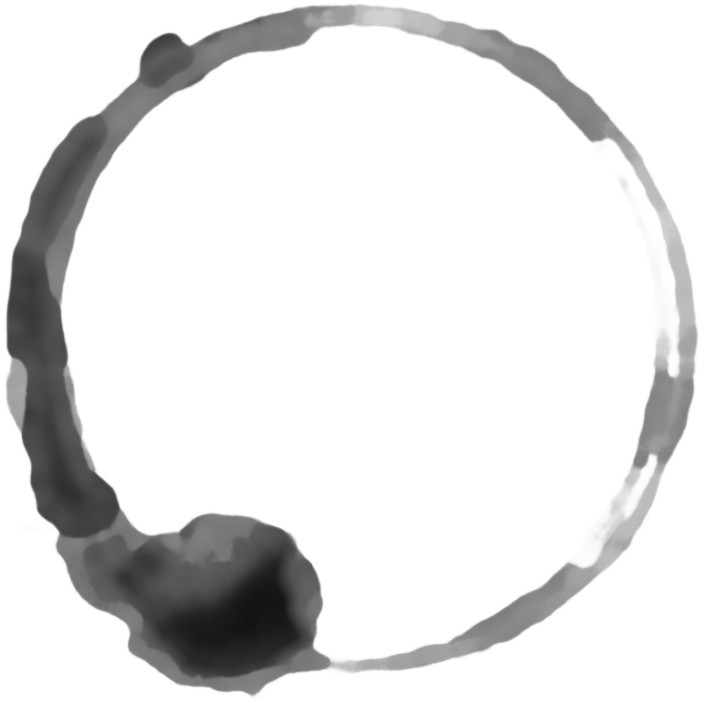
\includegraphics[width=0.3\textwidth]{imagenes/7/wine-stain.jpg}
\caption{Imagen del cuadro robado}
\label{fig:universe}
\end{center}
\vspace{-0.35cm}
\end{figure}

Antes de pasar a la siguiente sala, se implementó un pequeño script que detectaba cuándo el jugador interactuaba con los elementos que tapaban el cuadro, ya que debe retirarlos para llegar hasta él, y cuándo lo cogía. Este script sería más tarde integrado con el gestor de diálogos para que el vigilante hablara con el jugador mientras llegaba poco a poco su fin. Este script será descrito más adelante.

\subsection{Sala final y desenlace}

Para no terminar el juego tan abruptamente se decidió diseñar una última sala, con elementos como coches de policía, en la que el jugador tuviera un sentimiento de desenlace y de que el vigilante había sido apresando.

Finalmente, se decidió adaptar la antesala del museo, en la que había empezado todo, en la que se añadirían el resto de elementos. Aunque inicialmente se pensó que utilizar la misma escena que la antesala, finalmente se decidió que la sala final tenía la suficientemente autonomía e independencia como para ser una escena en sí misma.

En esta versión de la sala es de noche, para hacer ver al jugador que había pasado todo el día investigando para descubrir al ladrón, y hay varios coches de policía con las luces encendidas aparcados fuera que pueden verse desde los ventanales. Además, las luces del pasillo están encendidas y hay conos, balizas y una cinta de policía que impide la entrada al museo. La sala terminada puede verse en la figura \ref{fig:unity-sala-8}.

\begin{figure}[!h]
\begin{center}
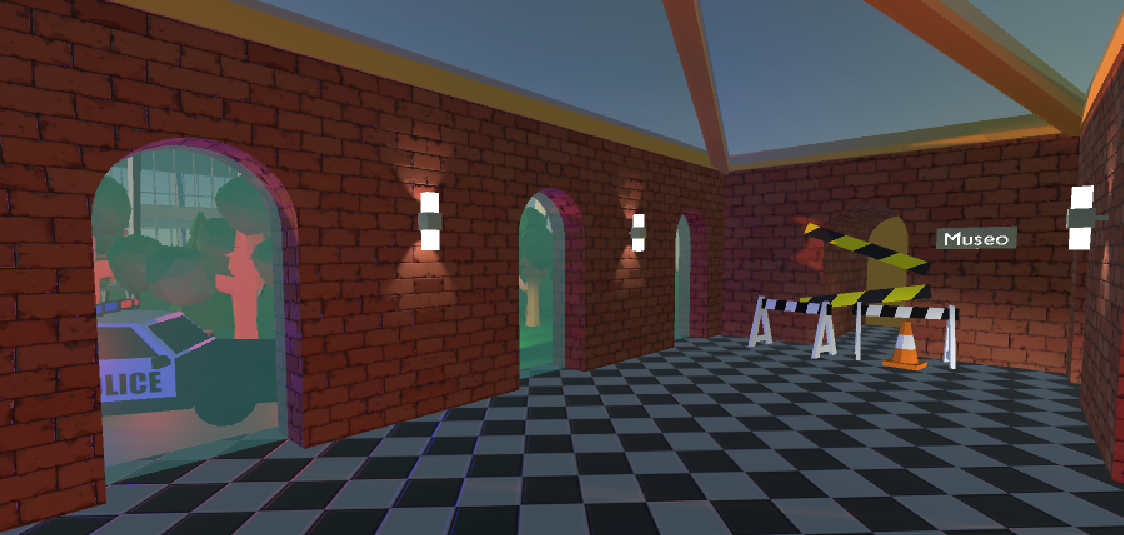
\includegraphics[width=0.85\textwidth]{imagenes/7/salas-unity/unity-sala-8.png}
\caption{Sala 8 renderizada en Unity}
\label{fig:unity-sala-8}
\end{center}
\end{figure}

Para el modelado de los coches de policía se ha usado el paquete de modelos de Unity \textit{Low Poly Police Car Pack}\footnote{\url{https://assetstore.unity.com/packages/3d/vehicles/land/low-poly-police-car-pack-59458}}, que puede ser descargado gratuitamente desde su tienda con licencia libre. Este paquete incluye varios modelos \textit{low poly} de coches de policía, lo que permite probarlos rápidamente en la escena y ver cuál queda mejor.

En esta sala, cuando el gestor de diálogos estuviera implementado, se recibiría una última llamada de la directora del museo agradeciéndole su trabajo y despidiéndose hasta la siguiente vez, abriendo la posibilidad a una segunda entrega del juego. 

\subsection{Modelo del vigilante y animaciones}

Como el vigilante juega un papel primordial en la narrativa del juego y su interacción con el jugador era constante, era necesario contar con una representación visual del mismo. Aunque inicialmente se barajó opciones mucho más simples, como utilizar una imagen bidimensional con un dibujo del mismo, totalmente estático, que simplemente estuviera en su sitio. Tras probarlo, el resultado no fue para nada convincente y fue evidente que había que utilizar un modelo tridimensional para el mismo. 

Al principio se buscaron modelos de ancianos con aspecto bonachón, para ocultar la cleptomanía del vigilante, pero aunque se encontraron algunas opciones perfectas, como los que se pueden ver en la figura \ref{fig:modelos-alt}, por \textit{3Dcartoon} (izquierda) y \textit{danielmgt} (derecha) costaban entre 80 y 120 euros, y como uno de los objetivos no funcionales de este proyecto era utilizar modelos gratuitos con licencia libre no fue posible usarlos.

\begin{figure}[!h]
\begin{center}
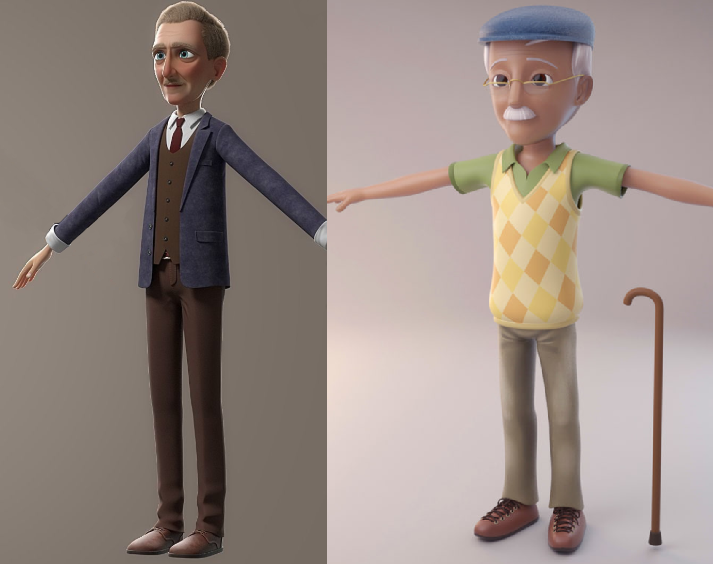
\includegraphics[width=0.6\textwidth]{imagenes/7/modelos-alt.png}
\caption{Algunos de los modelos que se valoraron para vigilante}
\label{fig:modelos-alt}
\end{center}
\end{figure}

En su lugar, y tas mucho buscar, se decidió utilizar el modelo de un hombre \textit{low poly} con licencia librel de Denys Almaral\footnote{\url{https://www.turbosquid.com/3d-models/3d-style-couple-casual-man-model-1387761}}, que se adaptó en Blender para hacerle parecer mayor, simplificar su topología y añadir elementos como la placa que tiene en el pecho, ajustar su esqueleto y cambiar el color de su ropa. Este modelo finalizado e importado ya ha podido verse en algunas de las salas anteriormente mostradas.

Tras ello, se importó a Unity se probó, pero era simplemente un modelo estático, lo que lejos de aportar realismo al juego se lo quitaba. Por ello, se decidió añadirle animaciones.

Unity está bastante bien preparado para utilizar animaciones; tiene integrada una herramienta capaz de importar y normalizar automáticamente esqueletos tridimensionales desde un modelo, utilizando una nomenclatura constante para los huesos. De este modo, es posible importar animaciones ya hechas al juego y aplicarlas a un modelo con un esqueleto normalizado para que, con relativamente poca configuración, sea posible utilizarlas con un resultado muy bueno.

Inicialmente se intentó implementar animaciones simples para el vigilante, pero mis habilidades como animador dejan mucho que desear y el resultado no era para nada convincente, por lo que se decidió importarlas ya hechas. El problema de las animaciones universales de Unity es que hay un mercado muy importante a su alrededor, y todos los paquetes medianamente completos que se encontraron eran de pago, llegando a costar cientos de euros. Por ello, ha sido necesario utilizar varios ejemplos de prueba con licencia libre, cada uno conteniendo una de las animaciones buscadas, como el paquete \textit{Idle MoCap} de Morro Motion para el estado de reposo del vigilante o el paquete \textit{Basic Motion} de 3D-Brothers para el saludo y la negación del guardia, por ejemplo.

Una vez que se importaron y se comprobó que funcionaban correctamente, se integraron en el juego. Para ello, lo primero que se hizo fue añadir un componente \textit{Animator} al objeto del vigilante, que relacionaba su esqueleto o \textit{avatar} en Unity con un \textbf{controlador de animaciones}.

Este controlador implementa una máquina de estados, asignando una animación a cada uno de ellos, y permite gestionar de un modo intuitivo las transiciones entre ellos. Como puede verse en la figura \ref{fig:animator}, que presenta en controlador de animaciones final de guarda, y en la que se ha seleccionado la transición desde el estado \textit{Greeting} hasta \textit{Idle}. A su derecha aparece la configuración de la transición, en la que podemos configurar cuánto durará la transición, en qué momento ocurrirá y qué \textbf{condiciones} han de darse.

\begin{figure}[!h]
\begin{center}
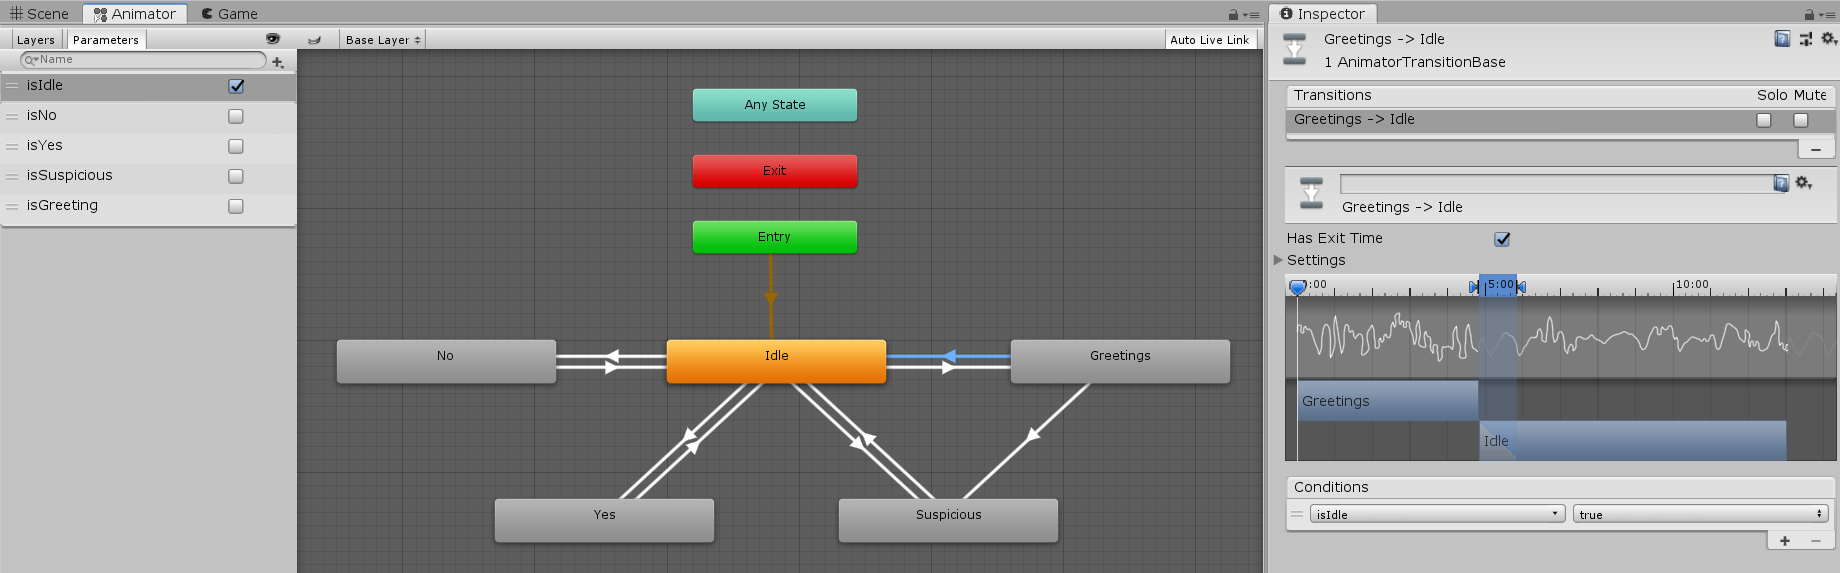
\includegraphics[width=1\textwidth]{imagenes/7/animator.png}
\caption{Máquina de estados del controlador de animaciones}
\label{fig:animator}
\end{center}
\end{figure}

Estas condiciones pueden configurarse a través de variables desde el propio editor, como puede verse a su derecha. En este caso, se ha asignado una variable booleana a cada transición, lo que permite activarlas cuando la variable cambia. En este caso el estado por defecto, en naranja, es \textit{Idle}, así que cuando la variable \texttt{isGreeting} sea \textit{true} la transición de estado hacia \textit{Greeting} se activará. Estas variables pueden modificarse desde el código fuente, lo que hace el controlador de animaciones una herramienta muy potente.

Estas animaciones están estrechamente ligadas con el sistema de diálogos; de hecho, es el propio gestor de diálogos el encargado de activar las animaciones. Por tanto, se explicará con más detalle en la siguiente sección.

\subsection{Implementación de un sistema de diálogos}

Como el guardia debía disponer de algún método de comunicar información al jugador, se ha diseñado un sistema de diálogos para ello. 

Como en el caso de las descripciones de los cuadros, y como ha podido verse en la figura \ref{fig:camera-overlay}, se ha utilizado un cuadro de texto superpuesto al mundo para que el jugador pueda leer lo que el guarda le dice. Además, como se explica más adelante, se ha añadido un efecto de sonido similar a los que utilizaban videojuegos antiguos para hacerlo más inmersivo.

Como el controlar el momento en el que se encontraba el guarda era muy complejo y abstracto, se ha implementado una máquina de estados para ello, que a su vez controla la animación que está reproduciendo el vigilante. El diagrama de la misma aparece en la figura \ref{fig:dialogs-state-machine}, y como puede verse hay 5 estados en total.

\begin{figure}[!h]
\begin{center}
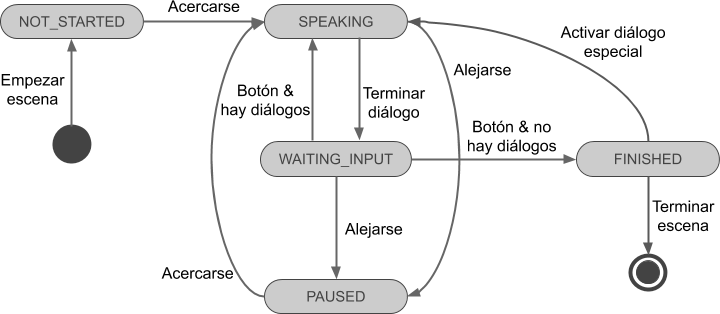
\includegraphics[width=1\textwidth]{imagenes/7/maquina-estados-dialogos.png}
\caption{Diagrama Máquina de diálogos del gestor de diálogos}
\label{fig:dialogs-state-machine}
\end{center}
\end{figure}

Al empezar el juego, el vigilante está callado y con la animación \textit{idle}, pero cuando el jugador se acerca a él (hecho que se detecta con una esfera de colisión), empieza a hablar con él. Cuando cada uno de los diálogos termina, se queda quieto esperando la interacción del jugador con el mando, y cuando pulsa empieza el siguiente diálogo. Sin embargo, cuando el jugador se aleja el guardia se callará hasta que vuelva a acercarse, momento en el que comenzará de nuevo el diálogo por el que iba. Cuando ha terminado todos los archivos de diálogo, pasa al estado terminado, en el que permanece hasta que la escena termina. A menos, claro, que se active algún diálogo especial, como una felicitación o una reprimenda por fallar alguna prueba, momento en el que volvería al estado de hablar.

Para los archivos de dialogo se ha utilizado la siguiente nomenclatura. Desde el punto de vista de la implementación, cada sala tiene una directorio en la que se encuentran sus diálogos, que comienzan por el numero 0, (e.g. \texttt{0.txt}), y aumenta una unidad para denotar el siguiente. Cuando no hay más archivos de texto, el gestor de diálogos lo da por terminado y pasa al estado \texttt{FNISHED}.

Además, se han añadido dos diálogos con la directora del museo, que es la que llama al detective para pedirle su ayuda. El primero sucede en cuanto el jugador entra en la antesala, con un retraso de 4 segundos, en la que le explica la situación y le indica que hable con el vigilante. El segundo ocurre en la sala final, con el mismo retraso, en el que le agradece la ayuda prestada. En ese momento, cuando el jugador termina de hablar con ella se desbloquea la puerta de salida del museo, y el jugador vuelve al menú principal.

Por otro lado, para no hacer que todo el texto apareciese de forma inmediata, se ha hecho que cada letra del texto aparezca cada dos décimas de segundo, intentando imitar la velocidad de un diálogo real. Para ello, y como puede verse en el listado \ref{lst:dialog-manager}, cada frame del juego se comprueba si el vigilante está hablando, y si sí se comprueba si ha pasado suficientemente tiempo como para mostrar otra letra. Si ya se han mostrado todas, se activa el estado de espera y se muestra un icono para que el jugador sepa que tiene que pulsar el botón correspondiente.

\begin{lstlisting}[caption=Fragmento del script del gestor de diálogos, label=lst:dialog-manager]
private void Update()
{
    if (speaking == SpeakingState.SPEAKING)
    {
        lastDeltaTime += Time.deltaTime;
        if (lastDeltaTime > TimeBetweetLetters)
        {
            if (currentLetterIndex < 
                    currentDialog.Length)
            {
                DialogObject.text = currentDialog.Substring(0, currentLetterIndex);
                currentLetterIndex++;
                lastDeltaTime = 0f;
            }
            else
            {
                speaking = SpeakingState.WAITING_INPUT;
                NextDialogIcon.SetActive(true);
            }
        }
    }
}
\end{lstlisting}

Por otro lado, para ejemplificar la integración con el controlador de animaciones con el gestor de diálogos, en el listado \ref{lst:animation-manager} se muestra cómo, desde el mismo script que anteriormente, se activa la animación de vigilante sospechoso, lo que se hace en la última y penúltima sala. En él, y como se ha explicado anteriormente, se utilizan las variables ligadas a las transiciones entre estados para activar determinadas animaciones. Uno de los problemas que se ha encontrado es que si simplemente se modifica la variable, la animación actual ha de terminar para que se active su transición; en cambio, si se obliga a reproducirla, como puede verse en la línea \ref{line:force-animm}, cambia automáticamente y sigue respetando las variables para decidir qué hacer cuando dicha animación termine.

\begin{lstlisting}[caption=Fragmento del script para activar animaciones, label=lst:animation-manager, escapechar=|]
public void ActivateSuspiciousAnimation()
{
    Animator animator = Guard.GetComponent<Animator>();
    if (animator)
    {
        animator.CrossFade("Suspicious", 0.5f);|\label{line:force-animm}|
        animator.SetBool("isIdle", false);
        animator.SetBool("isSuspicious", true);
    }
}
\end{lstlisting}

Este script, \texttt{DialogManager.cs}, ha resultado ser bastante extenso y complejo, y aunque tiene otras muchas partes interesantes, como la gestión de la interacción del jugador con el mando o de su acercamiento al vigilante dependiendo del estado, se deja al lector el consultarlo.

El resto del trabajo de los diálogos fue de índole narrativa para diseñar todos los diálogos a lo largo de las salas y los de confesión de vigilante, por lo que se omitirán. Si el lector los quiere leer, se encuentran en la ruta \texttt{Assets/Text/Dialogs}.

\subsection{Menú principal del juego}

Una vez que el juegos estaba prácticamente completo, se procedió a diseñar e implementar el menú del juego. Aunque inicialmente se pensó en hacer un menú 2D que no aprovechara el potencial de la \acs{VR}, al investigar se descubrió que el framework \acs{VRTK} soportaba los botones nativos de Unity, por lo que se decidió hacer un menú virtual.

Para ello, se ha tomado como referencia el menú principal del juego \textit{Beat Saber}\footnote{\url{https://beatsaber.com/}}, en el que el jugador se encuentra en un punto sin poder desplazarse, aunque puede move la cabeza, y utiliza láseres que salen desde sus mandos para señalar los botones que quieren pulsar, pulsando un botón para activar su selección. En un intento por lograr que hasta el menú del juego sea inmersivo, como en el caso del \textit{Beat Saber}, se ha decidido modelar una pequeña ciudad con edificios \textit{low poly} en la que el jugador se encuentra en el medio y desde la que ve tanto el propio museo desde fuera como varios botones tridimensionales con los que puede interactuar, como puede verse en la figura \ref{fig:main-menu}. Estos botones le permiten empezar una nueva partida, ver los créditos del juego o salir.

\begin{figure}[!h]
\begin{center}
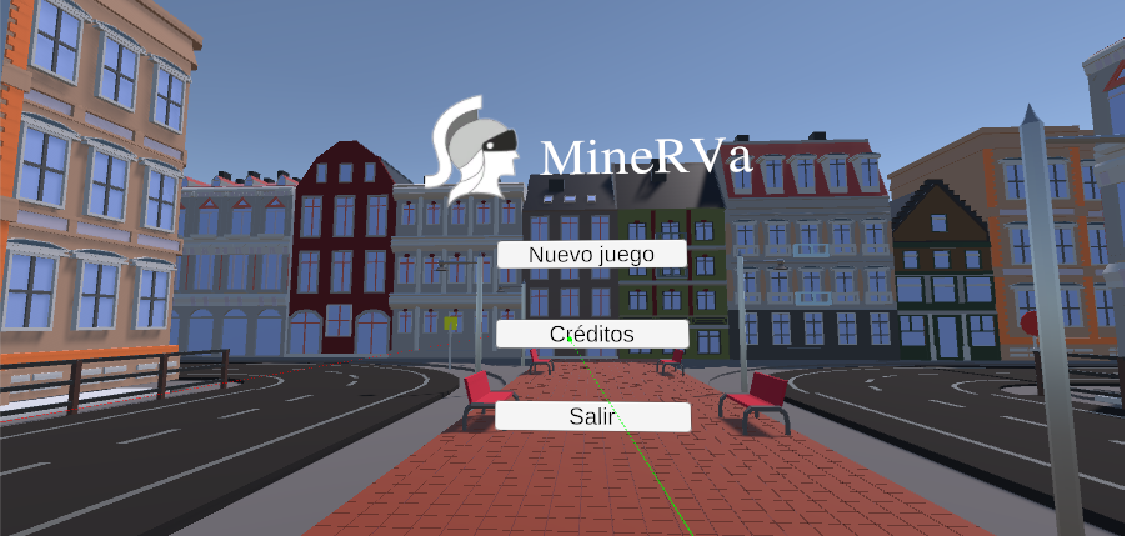
\includegraphics[width=0.85\textwidth]{imagenes/7/salas-unity/unity-menu.png}
\caption{Menú principal del juego}
\label{fig:main-menu}
\end{center}
\end{figure}

Como el modelar edificios es una tarea trivial, y el tiempo de la entrega estaba llegando a su fin, se decidió buscar paquetes de modelos que pudieran ser utilizados para este fin, y el paquete \textit{Low poly European City Pack} de karboosx, que contiene 8 edificios diferentes que coinciden con la estética del juego.

Tras ello se colocaron los botones y el logo del juego y se limitó la funcionalidad de los mandos para que el jugador no pudiera moverse con ellos. 

Tras ello, se creó el script \texttt{MenuManager.cs} desde el que se añadió un listener diferente a cada botón para poder controlar su funcionamiento. En el listado \ref{lst:menu-manager} se muestra un fragmento de este script, cómo se añade un listener al botón de salir y cómo este script comprueba si se trata del editor de Unity o del juego compilado para decidir qué hacer.

\begin{lstlisting}[caption=Fragmento del script gestionar el menú, label=lst:menu-manager]
private void Start()
{
    if (exitButton != null)
    {
        exitButton.onClick.AddListener(OnClickExit);
    }
}

private void OnClickExit()
{
    PlaySoundEffect();
    #if UNITY_EDITOR
        UnityEditor.EditorApplication.isPlaying = false;
    #else
        Application.Quit();
    #endif
}
\end{lstlisting}

\subsection{Música de fondo y efectos de sonido}

Por último, como el juego quedaba muy vacío y no había verdadera retroalimentación entre el jugador y su interacción, se decidió añadir música y efectos de sonido al juego.

Para toda la música se ha utilizado la página SoundImage\footnote{\url{https://soundimage.org/}}, un sitio web mantenido por donaciones que proporciona música gratuita y con licencia libre. A continuación se presenta una lista con la canción elegida para cada sala.

\begin{itemize}
    \item \textbf{Menú.} \textit{Magic Clock Shop}.
    \item \textbf{Antesala y sala 1.} \textit{Peaceful Evening}.
    \item \textbf{Sala 2.} \textit{Puzzle Game}.
    \item \textbf{Sala 3.} \textit{Clippity Clop}.
    \item \textbf{Sala 4.} \textit{Gentle closure}.
    \item \textbf{Sala 5.} \textit{Peaceful Mind}.
    \item \textbf{Sala 6.} \textit{Winding Down}.
    \item \textbf{Sala 7.} \textit{Thumbing Across Alaska}.
    \item \textbf{Sala 8.} \textit{The Jazz man}.
\end{itemize}

Además, para la música de la última sala, se ha utilizado Audacity para solapar sonido de sirenas de policía, ya que en esa sala hay coches de policía, como pudo verse en la figura \ref{fig:unity-sala-8}.

Para toda la música de fondo se ha usado el componente nativo de Unity \textit{Audio Source}, al que basta indicarle la canción que queremos reproducir, si ha de hacerlo en bucle y su volumen.

Por otro lado, se han añadido cuatro efectos de sonido distintos que se enumeran a continuación.

\begin{itemize}
    \item Cuando el jugador selecciona un elemento del menú, suena un pequeño click, añadiendo retroalimentación.
    \item Cuando alguien está hablando con el jugador, ya sea la directora o el vigilante, suena un efecto de sonido estilo \textit{8bit}. Este efecto se ha modificado en Audacity para hacerlo más grave en el caso del vigilante y más agudo en el caso de la directora, imitando la diferencia de tonos que suele haber entre voces de hombres y mujeres.
    \item Cuando la directora llama al jugador, ya que hablan siempre por teléfono, suena el timbre clásico de un teléfono.
    \item Por último, cuando el jugador activa la descripción de un cuadro suena un sonido de papel arrugado.
\end{itemize}

Como los efectos de sonido se reproducen en situaciones concretas, ha sido necesario activarlos de manera programática. Para ello, en los scripts que los utilizan, como el gestor de diálogos o el gestor de descripciones de cuadros, se ha añadido el código necesario para ello.

A modo ejemplificativo, en el listado \ref{lst:sound-effects} se muestra el código simplificado del gestor de diálogos que activa el efecto de sonido de una llamada. Como puede verse, recupera su componente para reproducir audio y detiene cualquier sonido que estuviera sonando. Más adelante y por convención, si el diálogo en cuestión contiene la palabra \textit{RING}, hace sonar el respectivo sonido al 5\% de volumen.

\begin{lstlisting}[caption=Fragmento del script para activar efectos de sonido, label=lst:sound-effects]
private void PlaySoundEffect(string dialog)
{       
    AudioSource audioSrc = GetComponent<AudioSource>();
    audioSrc.Stop();

    if (dialog.Contains("RING"))
    {
        audioSrc.PlayOneShot(ringSound, 0.05f);
    }
}
\end{lstlisting}

Finalmente, el resto de trabajo para esta entrega consistió en entregar los archivos de texto con las descripciones de los cuadros. Si el lector quiere leerlos, se encuentra en la ruta \texttt{Assets/Text/Painting\_descriptions}.

Como una de las tareas para la entrega final era grabar un vídeo mostrando el juego entero, no tiene sentido grabar otro enseñando los avances en esta entrega, ya que serían lo mismo, por lo que no se ha hecho.

\section{Entrega 7}

Esta última entrega se ha dedicado a realizar una evaluación del juego con usuarios reales, grabar un vídeo mostrando el juego entero, grabar y editar un tráiler del mismo, terminar de redactar e imprimir la documentación, realizar la presentación del proyecto para la defensa con tribunal.

\subsection{Evaluación con usuarios reales}